%%This is a Master Thesis template
\documentclass[a4paper,oneside]{report}
\usepackage{ucs}
\usepackage[T2A]{fontenc}
\usepackage[utf8]{inputenc}
\usepackage[english,bulgarian]{babel}
\usepackage{graphicx}
\usepackage{url}
\usepackage{textcomp}
\usepackage{amsmath}
\usepackage{amsfonts}
\usepackage{amssymb}

\addto\captionsbulgarian{%
  \renewcommand{\contentsname}%
    {Содржина}%
  \renewcommand{\tablename}%
    {Табела}%
  \renewcommand{\figurename}%
    {Слика}%
  \renewcommand{\bibname}%
    {Библиографија}%
  \renewcommand{\listfigurename}%
    {Листа на слики}%
  \renewcommand{\listtablename}%
    {Листа на табели}%
}




\begin{document}
\title{Архитектура и развој на мобилни апликации со знаење за контекстот}
\author{Томче Делев}
\date{Декември 2010}
\maketitle

{\flushleft{Ментор:}}\\
Вон. проф. д-р Дејан Ѓорѓевиќ\\
Факултет за електротехника и информациски технологии
\\[.5cm]
Комисија:\\
Проф. д-р Сузана Лошковска\\
Факултет за електротехника и информациски технологии
\\[.5cm]
Вон. проф. д-р Дејан Ѓорѓевиќ\\
Факултет за електротехника и информациски технологии
\\[.5cm]
Вон. проф. д-р Владимир Трајковиќ\\
Факултет за електротехника и информациски технологии


\newpage

\newpage
\begin{center}
{\Large{\it\textbf{Благодарност}}}
\\[2cm]
{\it
Би сакал да ја искажам мојата огромна благодарност до мојот ментор вон. проф.
д-р Дејан Ѓорѓевиќ за постојаната поддршка преку искреното пренесување на
неговото знаење и искуство, со што многу ми помогна во процесот на истражување и
изработка на овој магистерски труд. Исто така би сакал да искажам голема
благодарност до членовите на комисијата проф. д-р Сузана Лошковска и вон. проф.
д-р Владимир Трајковиќ за сите совети и знаења кои ми ги пружија во текот на
изработката на магистерскиот труд но и во текот на целокупните магистерски
студии.

Благодарност им должам и на колегите од компанијата CreationPal каде со
практична работа во областа на софтверското инженерство, а преку развој и
истражување на мобилната апликација SportyPal навлегов во оваа област.

На крај би сакал да искажам и огромна благодарност до мојата фамилија за
безрезервната љубов, огромното трпение и постојаното внимание што ми го
посветуваат во секој момент.
}
\end{center}

\tableofcontents
\listoffigures
\listoftables

\chapter{Вовед}
Денешните мобилни телефони се одликуваат со многу карактеристики со кој јасно се
издвојуваат како нова компјутерска платформа со зголемени можности за
пресметување. Тие претставуваат еден од нај значајните елементи кои ја
дефинираат третата ера во модерните компјутери. Првата ера на компјутерите ја
дефинираат компјутерите чие што време за пресметување е споделувано од страна на
многу корисници и организации наречени мејнфрејм компјутер. Втората ера ја
дефинира појавувањето на персоналниот компјутер кој начесто го поседува и
користи еден човек. Третата ера на модерни компјутери, ера на сеприсутно
пресметување се карактеризира со експлозијата на мали преносни компјутери во
форма на паметни телефони, лични дигитални помошници (PDAs) и вградени
компјутери во многу уреди кои ги користиме секојдневно. Сето ова создава еден
нов свет во кој секој користи и поседува повеќе компјутери. Напредокот во
компјутерската технологија постојано го зголемува бројот на компјутери кои се
интегрираат во секојдневниот живот на луѓето.

Можеби нај забележителен е напредокот кој се случува во развојот на можностите
за процесирање на мобилните уреди. Брзината на процесорот, големината на
работната меморија, капацитетот на постојаната меморија и брзината на мрежните
интерфејси постојано се развиваат и подобруваат. Овие уреди поседуваат
интегрирани камери кои се одликуваат со поголема резолуција, подобри оптички
карактеристики со што можностите за фотографирање се значително подобрени.
Постојат нови начини на поврзување (mini USB) и нови сензори со мала
потрошувачка. Акцелерометрите и жироскопите се веќе стандардни, а географско
лоцирање со помош на потпомогнат GPS (A-GPS), Wi-Fi или GSM е нешто што скоро
секој паметен телефон го овозможува. Исто така драматичен е и напредокот во
корисничкиот интерфејс кај мобилните уреди, пред се изразен преку интерфејсите
на допир (еднократен и повеќекратен), како и интерфејсот со чувствување на
движењето на уредот кој се популаризираа со појавувањето на iPhone.

Покрај сите иновации и напредокот кој е постигнат кај самите уреди, многу
значаен е напредокот во областа на оперативните системи и платформи за развој на
апликации за мобилни телефони. Во последните четири години се појавија платформи
како Android и iPhone кои за овој краток временски период се присутни кај повеќе
од 100 милиони корисници, а зголемувањето на оваа бројка е секојдневно и со
голема брзина. Денес развивачите на апликации за мобилни уреди може да избираат
меѓу iPhone, Android, Symbian, Ј2МЕ, Windows Mobile, BlackBerry, Brew и разни
други помалку познати софтверски платформи. Оваа сегментација на многу
софтверски платформи воведува многу предизвици за развивачите на апликации, но
претставува и мотив за постојан натпревар и иновации во оваа област.
Оперативните системи за овие уреди со сите свои можности но и со новиот концепт
на централизирани места (пазари) за апликации (iTunes, App Store, Android
Market, BlackBerry Marketplace, Nokia Ovi Store), ја менуваат перцепцијата на
корисниците за мобилните уреди: од едноставни телефони во мали, мобилни
компјутери, или како што ги опишува една нова кованица т.н. телефони за
апликации.

Мобилните уреди се со тенденција да бидат многу лични уреди. Тие се наменети да
ги носиме каде и да одиме. Нивната врска со корисниците е многу силна. Тие се
првото нешто кое го гледаме кога се будиме, ги користиме кога ни е досадно или
кога патуваме, а понекогаш преставуваат и главен извор на информации. Овие
карактеристики како и сите претходно опишани ги прават мобилните уреди многу
интересна тема за истражување во областа на сеприсутните пресметки (pervasive
computing). Основната идеја е дека моќните паметни телефони, а во исто време и
лични мобилни уреди во кохезија со многу други технологии, а преку користење на
напредните софтверски платформи ќе овозможат нова категорија на прилагодливи
апликации со знаење за контекстот на корисникот. Во
\cite{chen2000survey,baldauf2007survey}, е направен збир на истражувањето во
оваа област, а постојат и многу примери на апликации  и рамки за развој на
апликации со знаење за контекстот.


\section{Опис на проблемот}

Денес сме сведоци на огромен број мобилни апликации наменети за новите платформи
и најчесто наменети за групата на паметни телефони. Развивачите на овие
апликации се најчесто програмери кои поголемиот дел од своето искуство го имаат
во развој на апликации за персонални компјутери или во поново време веб
апликации во ерата на интернетот. Иако со иновациите во корисничкиот интерфејс
кој ги промовираат новите платформи за развој на мобилни апликации, корисничкото
искуство постојано се подобрува сепак најголем проблем на овие апликации
останува да се пронајде вистинскиот начин на развој на мобилна апликација која
ќе се вклопува во новата ера во која луѓето се во постојано движење и користат
многу компјутери. За некои од овие компјутери како што се паметните телефони и
се многу лични уреди, многу големо значење има вклучување на информации од
контекстот на корисникот во апликациите кои ги користи. Овие информации се пред
сè неговата локација, ситуацијата во која се наоѓа и други елементи од
контекстот кои мобилните апликации ги издигнуваат на едно повисоко ниво во однос
на апликациите за персонални компјутери и веб апликации со што ги прават многу
повеќе персонализирани.

Од аспект корисниците на мобилните уреди многу големо значење има контекстот во
кој се наоѓаат при користењето на овие уред. Контекстот на корисникот го
сочинуваат информации како локацијата, времето, опкружувањето или сите останати
елементи во неговата околина. Сите овие информации се од големо значење доколку
апликацијата знае за нив и може да го прилагоди своето извршување со што може да
понуди подобри сервиси и подобро корисничко искуство. Во овој магистерски труд е
презентиран процесот и методологијата на развој и архитектура на мобилни
апликации со користење на контекстот на корисникот. Развојот и архитектурата на
вакви апликации бараат истражување во области поврзани со собирање, обработка и
искористување на контекстот на корисникот.

Како резултат на истражувањето развиена е апликацијата наречена Гео Настани која
претставува систем за организација, споделување и промовирање на приватни и
јавни настани од различен карактер. Во оваа апликација се користи социјалниот
контекст на корисникот, односно неговите пријатели и врски, а се користи и
неговата локација но и други секундарни информации кои произлегуваат од
контекстот. Во описот на архитектурата и дизајнот направена е детална анализа на
архитектурните стилови кои може да се применат во ваков вид на софтверски
систем. Во процесот на развој направени се тестирања и евалуација на неколку
важни модули од архитектурата на системот, како што се методите за одредување на
локацијата на корисникот и начините на пренесување податоци меѓу различните
компоненти во системот.

Целта на апликацијата е да ги идентификува клучните аспекти во развојот на
современите мобилни апликации со знаење и употреба на контекстот на корисникот.
Гео Настани е софтверски систем кој помага во организирањето на настани, нивна
промоција, поканување на пријатели, препорака на интересни настани и слични
функционалности. Мобилната апликација со знаење на контекстот на корисникот
воведува многу дополнителни вредности на овој систем. Корисниците имаат постојан
пристап до системот каде и да се наоѓаат, може да пребаруваат настани во
зависност од нивната локација, да го означат своето присуство на некој настан,
како и да споделат информации во вид на кратки пораки или фотографии од самиот
настан корисни за другите корисници.

Придонесот на овој магистерски труд е во истражувањето и документирањето на
процесот на развој на современи мобилни апликации од аспект на идентификување на
најважните проблеми, предлог имплементација на нивни решенија, како и евалуација
на тие решенија. Идејата за софтвер за создавање записи и организација на
настани не е нова и е широко применета во многу системи на календари и друштвени
социјални мрежи. Но ниту една од овие апликации нема мобилна имплементација, а
уште помалку го идентификува користи или на каков било начин го вклучува
контекстот на корисникот. Затоа дел од придонесот е и самата имплементација на
апликацијата Гео Настани како прв обид за имплементација на мобилна апликација
за организација на настани со целосно вклучување на корисникот преку неговата
локација, пријатели и други контекстуални информации со што јасно се
идентификуваат придобивките и додадена вредност на целиот систем.


\chapter{Пресметување со знаење за контекстот}
 
\section{Вовед во пресметување со знаење за контекстот} 

Луѓето се многу успешни во пренесувањето идеи едни на други и во целиот процес
на остварување непосредна комуникација. Ова се должи пред се поради неколку
фактори како што се богатиот јазик за комуникација кој го користиме, потоа
општото познавање за светот и опкружувањето, како и имплицитно препознавање и
разбирање на секојдневни ситуации. Кога луѓето зборуваат меѓу
себе, тие ги користат овие информации и знаења, што е всушност контекстот. Во
ваквиот начин на комуникација сите овие информации ја зголемуваат продуктивноста
на разговорот. Меѓутоа, за жал способноста за споделување идеи не се пренесува и
во интеракцијата меѓу луѓето и компјутерите. Во традиционалната интеракција на
луѓето со компјутерите тие користат импровизирани механизми за пренесување на
информации до компјутерите. Како резултат на ова, денес компјутерите не се во
можност да го искористат контекстот во дијалогот човек/компјутер. Со подобрување
на знаењето за контекстот од страна на компјутерот, се збогатува интеракцијата
човек/компјутер со што се овозможува развој на многу покорисни и ефикасни
пресметковни сервиси. Со цел успешно користење на контекстот мора да се разбере
што всушност претставува контекстот од аспект на корисникот и од аспект на
апликацијата и кој се најдобрите начини да се обезбеди поддршка за искористување
на знаењето за контекстот. Соодветно разбирање на контекстот им помага на
развивачите на софтвер да изберат каков контекст ќе користат во своите
апликации, а разбирањето како контекстот може да се искористи помага во
одлучувањето какво однесување на основа на ова знаење ќе овозможи самата
апликација. 

\section{Што е контекст?}

Иако повеќето луѓе многу добро го разбираат зборот контекст и неговото значење,
сепак соодветна дефиниција е потребна за користење на контекстот во
компјутерските науки. Многу од дефинициите за контекстот може да се најдат во
претходна работа на оваа тема \cite{dey2001understanding,schilit1995system}.
Повеќето од дефинициите за контекстот се преку некое набројување на примери или
користење соодветни синоними на зборот.

Во својата работа \cite{schilit1994disseminating} во која прв пат го споменуваат
терминот знаење (свесност) за контекстот (context-aware), контекстот го
поистоветуваат со локацијата, идентификација на луѓето и објектите во
опкружувањето, како и менување на овие објекти. Со слична дефиниција во
\cite{brown1995stick} се дефинира контекстот како локацијата на корисникот,
опкружувањето, идентитетот и времето. Во \cite{dey1998context} контекстот се
дефинира како листа на неколку состојби, како емоционалната состојба на
корисникот, фокусот на неговото внимание, локацијата и ориентацијата, датумот и
времето и предметите и луѓето во неговото опкружување. Сите овие дефиниции го
дефинираат контекстот преку примери и тешко се применуваат во некои ситуации
кога треба да се одреди дали некоја информација која не е наброена во овие
примери за контекст може да се смета како дел од контекстот.

Во дел од речниците (Meriam-Webster) контекстот се дефинира како „меѓусебно
поврзани услови во кои нешто постои или се случува“. Многу од дефинициите
едноставно воведуваат синоними за контекстот, нарекувајќи го на пример,
ситуација или опкружување. Некои сметаат дека контекстот е опкружувањето на
корисникот, додека други сметаат дека е опкружувањето односно околината на
самата апликација. Во \cite{brown1996supporting} контекстот се дефинира со
елементите од опкружувањето на корисникот за кој компјутерот знае, во
\cite{franklin1998all} се смета на него како ситуацијата на корисникот, во
\cite{ward1997new} се поистоветува со состојбата на опкружувањето на
апликацијата, а \cite{rodden1998exploiting} го изедначуваат со прилагодувањата
на апликацијата. Како и кај дефинициите со примери, така и овие дефиниции
искажани преку синоними многу тешко може да се искористат во практика.

Сепак како збир на сето ова во \cite{schilit1994context} се истакнати најважните
аспекти на контекстот како што се: каде сте, со кој сте и што има околу вас. Тие го
дефинираат контекстот како околина на извршување која постојано се менува.
Елементи од кој е составена околината се:
\begin{itemize}
  \item Околината на извршување - број на процесори, уреди за внесување и приказ
  на податоци, можности на мрежата, поврзаност како и цена на пресметките
  \item Околина на корисникот - локација, луѓето во опкружувањето и социјалната
ситуација
  \item Физичката околина - осветлување и ниво на гласност
\end{itemize}

Во \cite{dey1998context} контекстот се дефинира како физичката, социјалната,
емоционалната и информациска состојба на корисникот, а во
\cite{pascoe1998adding} контекстот се дефинира како подмножество од физичките и
концептуалните состојби кој се од интерес за одреден ентитет. Овие неколку
дефиниции, иако се блиску до идеална дефиниција сепак се премногу конкретни.
Контекстот е всушност се она што е релевантно за апликацијата или за корисниците
на таа апликација. Меѓутоа не е возможно да се одреди кои аспекти од ситуацијата
или опкружувањето се релевантни, бидејќи ова се менува од ситуација до
ситуација. На пример во некои ситуации физичкото опкружување може да биде доста
значајно, а во некои други ситуации да биде сосема ирелевантно.

Конечно Day at. Al. во својата работа во
\cite{dey2000towards,dey2001understanding} даваат прилично задоволителна и општа
дефиниција за контекстот при што го дефинираат како:
\vfill
\emph{Секоја информација која може да се искористи за да се окарактеризира ситуацијата
на некој ентитет. Ентитет е личност, место, предмет кој се смета за релевантен
во интеракцијата меѓу корисникот и апликацијата, а ги вклучува и самиот корисник
и апликацијата.}
\vfill
Апликациите кои се свесни за контекстот ги обработуваат информациите како што се
кој, каде, кога и што (на пример, кој активности се случуваат) на ентитетите со
цел да одредат зошто некоја ситуација се случува. Самите апликации не одредуваат
сами од себе зошто некоја ситуација се случува, туку нивните развивачи ги
пишуваат на тој начин да го користат контекстот за да ја откријат намерата на
корисникот и соодветно да програмираат акции кои ќе ја задоволат таа негова
намера. На пример во апликација со знаење за контекстот која се користи за
информирање за возниот ред на градскиот превоз во некој град, кога корисникот ќе
се приближи до некоја постројка и ќе ја стартува апликацијата може да се
искористи неговата локација, како и времето од денот и да му се понудат
времињата на поаѓање кои ги поминале овие филтри и се релевантни за конкретниот
контекст. Притоа самата апликација ја препознава акцијата на корисникот, односно
неговото доближување до автобуска постројка (неговата намера), што означува дека
веќе е откриено зошто се случува тој настан и самата апликација одговара со
соодветна акција прилагодена точно на неговата намера.

При дефинирањето на контекстот никаде не се споменува дека тоа се исклучително
информации кои се добиваат имплицитно, што значи дека во самиот контекст
влегуваат и експлицитно внесени информации од самиот корисник. На пример,
идентитетот на самиот корисник може да се дознае имплицитно преку софтвер за
препознавање на лице на пример, но може и да биде внесен експлицитно ако го
запрашаме самиот корисник да го внесе неговото име притоа користејќи стандарден
интерфејс за внесување како тастатура. Од аспект на апликацијата и двете
информации се информации за идентитетот на корисникот и овозможуваат
дополнителни функционалности. Така како дел од контекстот се смета секоја
информација во апликацијата без разлика дали таа е собрана на имплицитен или
експлицитен начин. Сè додека на таа информација се реагира на некој начин во
апликацијата, самата апликација се смета дека го зема предвид контекстот и
станува апликација со знаење за контекстот. Во повеќето од апликациите се работи
на имплицитно собирање на информации за контекстот.

Постојат одредени видови на контекст, кој во практика, се поважни од останатите.
Ова се локацијата (каде), идентитетот (кој), времето (кога) и активноста (што).
Овие видови на контекст не само што се важни сами за себе со што одговараат на
прашањата каде, кој, кога и што, туку тие се извори и на многу други
контекстуални информации. На пример, ако е познат идентитетот на корисникот,
може да се дојде до дополнителни информации како неговите телефонски броеви,
адреса, е-адреса, место на раѓање, листа на пријатели, релации со други луѓе во
околината итн. Додека ако е позната неговата локација, можеме да одредиме што
друго се наоѓа околу него, кои луѓе и предмети се наоѓаат во близина или кои
настани се случуваат во близина. Меѓутоа целиот овој обид за категоризација на
контекстот е нецелосен и не доволно еднозначен. Како пример за ова може да
земеме информација за локацијата на корисникот. Нека неговата локација биде
некоја точка во некоја соба. Ова локација може да се дефинира со координатите во
самата соба, преку самата соба, преку спратот на кој се наоѓа собата, преку
зградата во која се наоѓа, преку градот, итн. Сè уште не е јасно како оваа
категоризација може да помогне во градењето на хиерархиско знаење за контекстот.
Како ќе се репрезентира и како ќе се моделираат информациите за контекстот е
уште едно отворено прашање на кое многу истражувачи му посветуваат внимание.

\section{Категоризација на апликациите со знаење за контекстот}
Во подетални истражување на апликациите со знаење за контекстот направена е
категоризација во однос на нивните можности. Постојат три обиди за создавање на
ваква поделба. Првата [12] има две ортогонални димензии: дали тоа што треба да
се изврши е да се добијат некакви информации или треба да се изврши некоја
акција и дали извршувањето е рачно или автоматско. Апликациите кои користат
одредени информации од контекстот на корисникот со цел да му понудат листа со
избори во зависност од тие информации се класифицирани како апликации со
приближен избор. Приближно избирање е техника на интеракција во која се
презентира листа на предмети (печатачи) или места (банки) при што нештата кои се
релевантни за контекстот на корисникот се обележани и полесно е да се изберат.
Апликациите кои автоматски ги прибираат информациите за корисникот и се
засновани на неговиот контекст се класифицирани како апликации со автоматска
контекстуална конфигурација. Тоа е техника на ниво на системот која креира
автоматско поврзување со одреден ресурс врз основа на моменталниот контекст.
Апликациите кои извршуваат акции поттикнати од самиот корисник и тоа врз основа
на контекстот се класифицирани како апликации со контекстуални акции. Тоа се
сервиси кои може да се извршат само кога корисникот се наоѓа во одреден контекст
и само тогаш се појавуваат. Како последни се апликациите кои извршуваат акции
автоматски наместо корисникот врз основа на дадените контекстуални информации со
што користат контекстуално поттикнати акции. Тоа се сервиси кои се извршуваат
автоматски кога ќе се случи одредена комбинација на контекстот а се базираат на
едноставни ако/тогаш правила.

Малку понова е поделбата предложена во [13]. Иако постои значително преклопување
со претходната поделба, сепак постојат и некои важни разлики меѓу двете поделби.
Оваа поделба пред сè е наменета на најважните својства на контекстот, наспроти
претходната, која идентификува различни класи на апликации со знаење за
контекстот. Во реалноста, следните својства на контекстот се пресликуваат во
класите на апликации во претходно предложената поделба [12]. Првото својство е
собирање на контекстот и претставува можноста преку користење на системот од
сензори што го поседува уредот да се идентификуваат контекстуални информации и
истите да му се презентираат на корисникот. Ова е слично со приближниот избор,
освен што во овој случај, не е неопходно корисникот да избере некоја од
контекстуалните ставки за повеќе информации. Следното својство е прилагодување
во зависност од контекстот и претставува можност за автоматско извршување или
изменување на некој сервис врз основа на моментниот контекст. Ова својство
директно се пресликува со контекстуално поттикнатите акции. Третото својство,
контекстуално откривање на ресурси, овозможува апликациите со знаење за
контекстот да лоцираат и искористуваат ресурси и сервиси кои се релевантни за
корисничкиот контекст. Ова директно се пресликува со својството на автоматско
контекстуално конфигурирање. Последното својство, контекстуално збогатување, е
можноста да се поврзуваат дигитални податоци со корисничкиот контекст. На
пример, корисникот може да направи виртуелна забелешка со детали за расипан
телевизор и истата да ја прикачи на телевизорот. Кога друг корисник е во близина
на телевизорот и се обидува да го користи, тој ќе ја забележи виртуелната
белешка која е оставена претходно. Ова својство не постои во претходната
класификација.

И во [12][13] се наброени можности за искористување ресурси релевантни за
контекстот на корисникот, можноста за автоматско извршување команди врз основа
на контекстот и можноста за прикажување релевантни информации на корисникот.
Притоа во [13] се оди и чекор понатаму со тоа што е додадено и својството да се
прикажуваат релевантни информации на корисникот со вклучување и прикажување на
делови од самиот контекст, а не само информацијата потребна да се направи
изборот (на пример, прикажување на локацијата на корисникот наспроти прикажување
на листа на печатачи и можност на корисникот да избере еден). Втората поделба
има категорија која не постои во првата поделба: контекстуално збогатување, или
можноста да се поврзат дигитални податоци со контекстот на корисникот. Исто така
и втората поделба не подржува прикажување на акции релевантни на контекстот на
корисникот, како што тоа е овозможено преку контекстуалните акции во првата
поделба.

Во [14] се комбинираат идеите од овие две поделби, а се земаат предвид и три
значајни разлики. Слично со втората поделба, тоа е листа на својства на
контекстот кои можат да се поддржат во апликациите со знаење за контекстот.
Постојат три категории: 

\begin{enumerate}
  \item Презентација на информации и сервиси на корисникот
  \item Автоматско извршување на сервиси
  \item Означување на контекстот со информации за понатамошно пребарување
\end{enumerate}

Презентацијата е комбинација на приближното избирање и контекстуалните акции, а
додаден е и делот за презентирање на контекстот (во форма на информација) на
корисникот. Пример на ова прво својство е мобилен компјутер кој динамички ја
обновува листата на најблиски печатачи во моментите кога корисникот се движи во
зградата. Автоматското извршување е исто како и контекстуално поттикнати акции и
контекстуалното прилагодување. Примери на второто својство се кога на корисникот
му се печати документ на најблискиот печатач до него, или кога на пример аларм
се активира кога на некоја далечна локација се покачила температурата над некоја
граница или кога автоматски се испраќа кратка порака кон пријател кога тој/таа е
на одредено растојание од корисникот. Означувањето може да се поистовети со
контекстуалното збогатување. Пример за ова е кога апликацијата ги запишува
имињата на документите кои ги отпечатил корисникот, времињата кога тие се
отпечатени како и моделот на печатач кои ги печател. Понатаму корисникот може да
се повикува на овие информации кога ќе има потреба да одреди каде биле
отпечатени тие копии и каде ги има заборавено.

Последната поделба има две значајни карактеристики кои ја одделуваат од
останатите: одлуката да не се прави разлика меѓу информациите и сервисите и
отстранувањето на искористување на локалните ресурси од листата на својства. Во
повеќето случаи, прилично е тешко да се направи разлика помеѓу презентација на
информација и презентација на сервис. На пример, кога се работи за листа на
печатачи кои се подредени по нивната близина до корисникот, тоа е пример на
давање информација на корисникот. Но дали таа листа е листа на информации или
листа на сервиси зависи од тоа како всушност корисникот ја користи таа
информација. На пример, ако корисникот само ја погледне листата да се запознае
со печатачите во негова близина, тогаш ја користи како информација. Меѓутоа, ако
корисникот избере печатач од листата за да го користи, тогаш листата се однесува
на сервиси. Затоа наместо да се претпоставува намерата на корисникот,
информациите и сервисите се третираат на ист начин.

Оваа поделба исто така не ја користи експлоатацијата на локални ресурси или
откривањето на ресурси како својство на контекстот, но го вклучува како дел од
првите две категории. Откривањето на ресурси е можноста да се лоцираат нови
сервиси знаејќи за контекстот на корисникот. Оваа можност може да се смета како
сосема иста како и изборот на сервиси врз основа на контекстот. На пример, кога
корисник влегува во канцеларија, неговата или нејзината локација се менува, а и
листата на печатачи во близина се менува. Листата се менува со што се додаваат
печатачи, се вадат, се преуредуваат (на пример, според нивната близина). Ова е
пример на откривање на ресурси или едноставно презентација на сервиси и
информации? Наместо откривањето ресурси да се категоризира во посебна
категорија, поделено е во две постоечки категории: презентација на информации и
услуги на корисникот и автоматско извршување сервиси. Кога апликацијата
презентира некоја информација на корисникот, тогаш припаѓа на првата категорија,
а кога автоматски извршува некоја услуга припаѓа на втората категорија.

Дефинициите на контекстот им овозможуваат на истражувачите да одредат дали
некоја апликација го користи или не го користи контекстот. Ова е корисно за да
се одреди на какви видови апликации треба да се фокусираат. Категоризацијата на
својствата на контекстот дава две главни придобивки. Првата е што уште повеќе се
специфицираат видовите апликации во зависност на нивното користење и знаење за
контекстот. Втората придобивка е тоа што опишува видови својства на кои треба да
се посвети посебно внимание во процесот на развој на апликации со знаење за
контекстот.
\begin{figure}[htb]
\centering
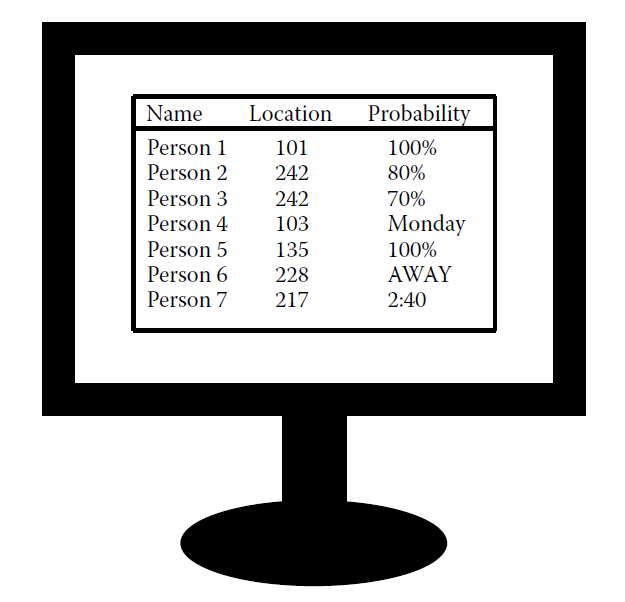
\includegraphics[scale=0.4]{images/active_badge}
\caption{Приказ од оригиналната апликација „активна значка“ кон локацијата со
соодветната веројатност на носителите на „Активна Значка“}
\label{fig:active_badge}
\end{figure}

\section{Апликации со знаење за контекстот}

Во овој дел ќе бидат опишани некои историски значајни апликации со знаење за
контекстот со кои започнува оваа област, како и некои по современи примери на
апликации во кои може да се препознае користење на контекстот.

Една од првите апликации која се смета дека прва активно го разгледува и користи
контекстот на корисникот е системот Активна значка (Active Badge) [15]. Во оваа
апликација (Слика 1) корисниците носат Активни значки, со инфрацрвени
трансмитери кои испраќаат уникатен идентификациски код. Како што корисниците се
движат низ нивната зграда, базата на податоци се менува динамички со
информацијата за локацијата на секој од корисниците, најблискиот пристап до
телефон, како и веројатноста дека ќе најдете некој на таа локација (врз основа
на староста на податоците). Кога ќе се добие повик за одреден корисник,
рецепционерот ја користи базата на податоци да го пренасочи повикот кон
последната локација на која е забележан корисникот, наместо само слепо да го
пренасочи повикот кон канцеларијата на корисникот во која тој можеби и не се
наоѓа. Оваа апликација, заедно со многу други од првичната работа во полето на
пресметувањето со знаење за контекстот се фокусирани на пресметување со знаење
на локацијата на корисникот. Ваквите апликации денес се познати и како
локациски-базирани апликации или сервиси.

Втората почетна работа во оваа област е изработена од Ubicomp group во Xerox
Palo Alto Research Center (PARC) во раните 1990ти. Во нивната работа [12] го
воведуваат терминот знаење за контекстот и развиваат архитектура на систем за
поддршка и развој на апликации со знаење за контекстот како дел од нивната
влијателна работа PARCTAB [16]. Во овој систем информациите им се презентираат
на корисниците во зависност од нивната близина до сервисите (на пример, печатачи
и луѓе), уредите се вклучуваат или конфигурираат врз основа на луѓето кои се
наоѓаат во близина, се презентираат информации или сервиси врз основа на
локацијата на корисникот и автоматски се извршуваат сервиси на начин кој зависи
од движењето или близината на корисниците до одредени соби или уреди.

Од тогаш наваму, постојат многу примери на апликации во кои е применето знаењето
за контекстот и истите се имплементирани во огромен број на домени. Сепак во
пракса се издвојуваат три главни класи на апликациски домени и тоа: туристички
водичи, системи за потсетување и контрола на околината.

\subsection{Мобилни туристички водичи}

Мобилниот туристички водич е најчестиот и нај типичен пример на апликација со
знаење за контекстот. При интеракцијата на корисникот со еден ваков систем кога
тој посетува некој музеј или град тој со себе носи преносен компјутерски уред.
Како што корисникот се движи на различни локации, неговиот мобилен уред
прикажува информации релевантни за тие локации. Иако првичните системи прилично
се базираат на локацијата [17][18], некои подоцнежни системи ги земаат предвид и
интересите на корисникот како и времето кое корисникот сака да го помине на
одредена туристичка локација или колку време може да потроши корисникот за
одредена туристичка тура [6][19].

\subsection{Потсетници} 

Вториот пример на типични апликации со знаење за контекстот се системи
потсетници. Потсетниците со знаење за контекстот презентираат потсетници на
корисникот, поттикнати од некои измени во контекстот. Алармниот часовник е една
од нај познатите вакви апликации и функционира со користење на едноставен
контекстуален активатор, време, да вклучи аларм, едноставна форма на потсетник.
Слично, локациски-базирани сервиси може да поттикнат некои потсетници кога
корисниците се на одредена локација или се на некое растојание еден од друг [4].
По софистицирани потсетници користат комбинација од различни форми на контекст
да вклучат некои потсетник. Со тоа што се по софистицирани, овие апликации може
да ги потсетуваат корисниците на по соодветен начин, со што го вклучуваат
вистинскиот потсетник во вистинската ситуација [14][20].

\subsection{Контрола на околината} 

Третиот вид на апликации со знаење за контекстот е систем за контрола на
греењето, осветлувањето или други својства на околината, со цел да се подобри
ефикасноста и да се постигне одредена заштеда на енергија. Како што луѓето сè
повеќе без потреба ги оставаат вклучени светлата, или треба рачно да го менуваат
нивото на затоплување или ладење за да се чувствуваат удобно, развиени се многу
системи кои во овие случаи ја преземаат контролата од корисникот. Некои се
засновани на прилично едноставни правила [21], додека некои други користат многу
пософистицирани методи како некои техники на машинско учење за да научат како
корисниците го користат просторот и соодветно ги постават нивото на затоплување
и осветлување [22].

\subsection{Современи апликации со знаење за контекстот}

Иако овие апликации од денешен аспект можеби изгледаат доста едноставно, сепак
вакви апликации се уште се развиваат од страна на истражувачите, а што е уште
позначајно многу од овие апликации почнуваат да излегуваат од светот на
истражувањето и да се претвораат во комерцијални апликации кои се широко
распространети. Покрај трите основни домени, истражувачите и развивачите
развиваат апликации во многу различни домени вклучувајќи ги следните:

\begin{itemize}
  \item Меѓусебна комуникација со кратки пораки [23]
  \item Вознемирување додека сме во канцеларија или додека сме мобилни [24]
  \item Телефонски повици [25]
  \item Здравствена заштита [26]
  \item Локациски-базирани системи
  \item Персонализација на апликации [27]
  \item Периферни прикази на информации [28]
\end{itemize}  

Ова е една огромна листа и наместо да се надополнува или пак да се зборува за
деталите на овие апликации, при што сето ова може да биде веќе застарено многу
скоро, многу е важно да се напомене дека истражувањето во ова поле е во добра
насока. Со самото тоа што се движи од апликации за помалку корисни работи и игри
со мал придонес за реални корисници во реални ситуации кон по фундаментални
проблеми кои се однесуваат на сите аспекти од секојдневниот живот и критични
ситуации. Ова поле ја помина фазата на зреење и сега истражувачите и развивачите
го посветуваат нивното внимание не само прикажувајќи што може да се направи и
што сè е можно, туку на она што е по убедливо и заслужува поголемо внимание.

Уште еден значаен момент е и забелешката дека голем број на истражувачи работат
на развој на апликации со знаење за контекстот, но нивниот фокус не е
контекстот. Тие едноставно развиваат корисни, значајни апликации кои едноставно
случајно го користат и контекстот. Иако ова може да се смета и како мала
дискриминација, сепак знаењето за контекстот ќе достигне ниво на зрелост кога
често на него ќе се гледа како на една од можностите на апликацијата, а не
нејзин основен фокус.

Еден од поинтересните примери за современа мобилна апликација со знаење за
контекстот е мобилна апликација која служи како личен тренер во извршувањето на
секојдневни физички активности. SportyPal [29] е токму ваков вид на мобилна
апликација во која контекстот на корисникот е всушност основната идеја во целата
апликација. Во оваа апликација корисниците избираат некоја спортска активност
како трчање, одење, планинарење или возење велосипед, по што апликацијата
постојано го следи и снима нивното движење. Исто така им пресметува моментална
брзина на движење, поминато растојание и потрошени калории. Во овој вид на
апликации контекстот го претставува локацијата на корисникот како и нејзиното
менување преку постојаното движење на корисникот. Ова е пример на апликација во
која единствено преку следење и запишување на информациите за контекстот на
корисникот може да се имплементира современа и корисна мобилна апликација. Втор
интересен пример на современа мобилна апликација со знаење за контекстот е
апликацијата Locale [30] во која во зависност од контекстот на корисникот
автоматски се нагодуваат прилагодувањата на мобилниот телефон. Се врши
прилагодување на начинот на ѕвонење, осветленоста на екранот, безжичните мрежи и
други нагодувања кои се директно засегнати од елементите на контекстот на
корисникот како локацијата, времето од денот, амбиентот во просторијата и други.

\section{Дизајн и имплементација на апликации со знаење за контекстот}

Во овој дел е опишан начинот и алатките кои постојат за дизајн и имплементација
на апликации со знаење за контекстот.

\subsection{Процес на дизајн}

Процесот на дизајн на повеќето од апликациите со знаење за контекстот може да се
сведе на прилично едноставна идеја: откривање и одредување на видот на
контекстот кој и е потребен на вашата апликација, кога го примате тој контекст и
што сакате да правите со него. Сепак, потребно е уште малку повеќе работа за да
се развие апликација со знаење за контекстот претставена преку чекорите на
Табела 1. Првиот чекор во развојот е спецификацијата на контекстот - одредување
на кои елементи од контекстот ќе се обработуваат во апликацијата и што ќе се
извршува во самата апликација врз основа на овие контекстуални информации.

Табела 1. Чекори во развојот на апликацијата за споделување на активноста во
оддалечена просторија 

Чекор   Пример Спецификација Вклучување различно обоени ЛЕД диоди (црвена, жолта, зелена) во зависност од
нивото на активност во оддалечената локација Преземање   Пишување софтвер за
анализирање на промените на сликите (frame-by-frame) од видео камера од
оддалечена локација и инсталација на камерата Прием   Објавување на информации
како нивото на активност кои може да се искористат во други апликации со
користење на пристапот со објавување/пријавување Испорака    Апликацијата сака
да ги прими сите промени на активноста над одредено ниво Акција  Апликацијата ги
анализира примените промени на активноста и ги вклучува соодветните ЛЕД диоди
(црвена, слаба активност; жолта, средна активност; зелена, висока активност)

Овој чекор вообичаено се прави преку проучување на доменот на апликацијата,
нејзините корисници и одредување кои сервиси би било корисно да им се понудат.
Вториот чекор е преземање на контекстот - одредување кој вид на хардвер и
софтвер се потребни да се собере контекстот одбран во првиот чекор. Ова вклучува
инсталација на софтверот на соодветната платформа, детално запознавање со
видовите информации кои ги овозможува сензорот, искористување на апликациски
интерфејс за програмирање (API) (ако постои) за комуникација со сензорот,
одредување на начинот на кој ќе се чита сензорот и како ќе известуваме за сите
промени на сензорот. Исто така, доколку е возможно, податоците од контекстот се
запишуваат и се комбинираат со други податоци, а се применува и учење и
одлучување за да се дојде до знаење за ситуацијата на повисоко ниво. Третиот
чекор е испорака на контекстот - спецификација како ќе се пренесе контекстот од
сензорите (кои може да се на оддалечена локација) до апликациите кои ќе го
користат контекстот. Четвртиот чекор е прием на контекстот - во кој апликациите
специфицираат кој контекст им е потребен (можно е и спецификација од кои
сензори) и примање на соодветниот контекст. Ова вклучува претворање на
контекстот во форма која е корисна од страна на апликацијата преку негова
интерпретација, а потоа и соодветна анализа дали овој контекст во комбинација со
други информации, опишува релевантна ситуација за корисникот и за апликацијата.
Последниот чекор е акцијата - анализирање на севкупниот контекст кој е примен и
одредување која акација треба да се изврши и извршување на таа акција. Иако
апликациите може да се многу по сложени од ова, сепак повеќето апликации се
опишуваат преку овој едноставен процес на дизајн.

\subsection{Алатки за развој}  

Врз основа на предложениот процес на дизајн, развиени се неколку алатки или
софтверски архитектури за поддршка на развојот на апликации со знаење за
контекстот. Ако за првиот чекор на спецификација може да се каже дека е
задолжителен во развојот на сите апликации, останатите чекори може да се
избегнат во зависност од тоа што овозможува алатката која се користи за развој.
Во најдобар случај, спецификацијата на ситуациите од интерес и соодветните
контекстно базирани однесувања се доволни за контекстот да се пренесува од
соодветните сензори до апликациите, со соодветно резонирање и интерпретација, а
потоа и соодветно извршување на акција.

\begin{figure}[htb]
\centering
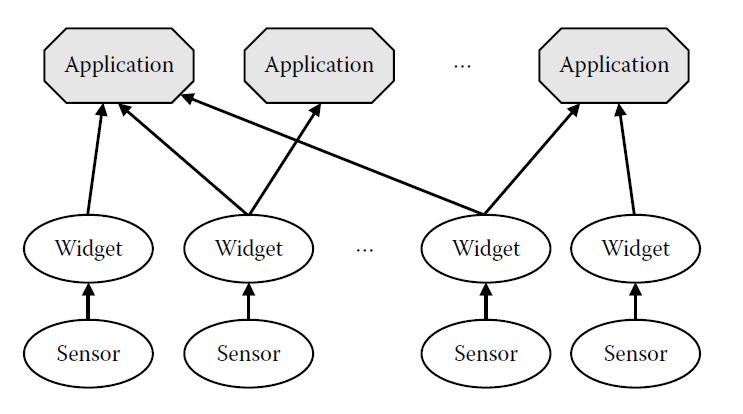
\includegraphics[scale=0.4]{images/widget_based}
\caption{Систем за развој на апликации со знаење за контекстот заснован на
објекти (widgets)}
\label{fig:widget_based}
\end{figure}
 
Постојат три основни алтернативи кои се користат за развој на апликациите: без
поддршка, систем заснован на објекти (Widgets) прикажан на Слика 2 и систем
заснован на школска табла (Blackboard). Поголемиот дел од системите, посебно тие
развиени пред 1998, се развиени без соодветна архитектура или со голема
прилагодливост кон мало множество на апликации. За секоја од овие апликации,
целосниот процес на дизајн мора да се примени поединечно за секоја од нив. Многу
малку, ако и воопшто некаков изворен код може повторно да се искористи меѓу
различни апликации, така што поголем дел од изворниот код е прилагоден за секоја
од апликациите соодветно.

Основниот пристап со објекти се
заснова на моделот на развој на графичките кориснички интерфејси (GUIs). Во
раните 1980ти, не постоел генерален модел за справување со корисничките податоци
и не постоела можност за повторно искористување на објекти кои би се справувале
со тоа. Во средина на 1980тите, се појавуваат првите GUI алатки кои поддржуваат
повторно искористување, притоа вклучувајќи ја во себе севкупната инфраструктура
за справување со настаните при внесување податоци и библиотека на компоненти што
може да се користат во повеќе различни апликации. Овие алатки го олеснуваат
развојот на графичките кориснички интерфејси со овозможување на следните
придобивки:

\begin{itemize}
  \item Тие ги сокриваат спецификите на уредите за физичка интеракција
од програмерот на апликацијата со што овие уреди може да се менуваат и притоа
настанатите промени да немаат големо влијание на апликациите. Дали корисникот
покажува или клика со глувче или покажува и допира со прсти или користи
скратеници од тастатура не предизвикува никакви измени во апликацијата.
\item Се справуваат со деталите на интеракција за да и овозможат на апликацијата
релевантни резултати од акциите на корисникот. Апликациите едноставно треба да
имплементираат некоја функција во која се враќа резултатот од интеракцијата на
корисникот.
\item Овозможуваат градбени блокови за презентација кои може да се
искористуваат и комбинираат во повеќе апликации. Тие претставуваат апстракција
на изгледот и однесувањето, а програмерот не треба да знае како се изградени за
да ги користи.
\end{itemize}

На сличен начин, во доцните 1990ти и раните 2000ти, се појавуваат софтверски
алатки за управување со контекстот како што се Context Toolkit [31] и Java
Context-Aware Framework [32] кои на сличен начин го прилагодуваат овој модел на
објекти енкапсулатори на однесување и акции. Контекст виџет е софтверска
компонента која овозможува апликациите да пристапат до контекстни информации од
нивната извршна околина. На ист начин како што GUI виџетите ги изолираат
апликациите од презентациски работи, така контекст виџетите ги изолираат
апликациите од работи како преземање на контекстот преку обезбедување на
стандарден интерфејс кон сензорите. Контекст виџетите ги овозможуваат следните
предности:

\begin{itemize}
  \item Овозможуваат издвојување на засебните и концептуално
различни делови со што ја сокриваат комплексноста на сензорите кои се користат
во апликацијата. Дали присуството на луѓето се забележува со користење на
активни значки, сензори на подот, обработка на слики или комбинација од нив нема
влијание во дизајнот на апликацијата.
\item Тие ги апстрахираат контекстуалните
информации да одговараат на барањата на апликациите. Виџет кој ја следи
локацијата на корисникот во некоја зграда или град ја известува апликацијата
само кога корисникот се движи од една соба во друга или кога од една улица
преминува на друга, а не известува за помалку значајни движења. Со неколку
зборови овозможуваат апстрахирани информации кои очекуваме дека се најпотребни
во самата апликација.
\item Овозможуваат едноставен пристап до контекстни податоци
преку механизам на пребарување и нотификација (на пример објави/пријави)
овозможен преку стандарден интерфејс за пристап на контекстот. Без разлика каков
контекст се собира од околината, сите виџети го овозможуваат на ист начин.
\item Овозможуваат градбени блокови за восприемање на контекстот кој се прилагодливи и
може повторно да се искористуваат. Виџет кој ја следи локацијата на корисникот
може да се користи во многу различни апликации, од туристички водичи се до
системи за следење на канцелариски простории. Понатаму, овие виџети може да се
комбинираат слично како и GUI виџетите. На пример, нека постои виџет кој
забележува присуство на луѓе во просторија. Над овој виџет може да се развие нов
виџет кој ќе забележува состанок кога ќе се забележи присуство на повеќе од еден
човек во просторијата. 
\end{itemize}

Како додаток на контекст виџетите, оваа инфраструктура овозможува компоненти за
комбинирање на контекстни информации, извлекување на заклучоци на повисоко ниво
од контекстот на пониско ниво, собирање и групирање на контекст од различни
извори и откривање на соодветни компоненти. Како колекција, виџетите не само што
овозможуваат компоненти кои може да се искористат за развој на поединечни
апликации, туку служат и како дистрибуирана инфраструктура која може да
поддржува повеќе апликации истовремено. Ова е пристап кој е се повеќе застапен
во реални софтверски пакети, а и доста популаризиран со самото вклучување на
апликациски интерфејс за програмирање (API) за сензорската и локациската
платформа во Microsoft Windows 7 кој овозможува пристап до сензори за локација и
осветленост и овозможува развој на апликации со знаење за контекстот.

\begin{figure}[htb]
\centering
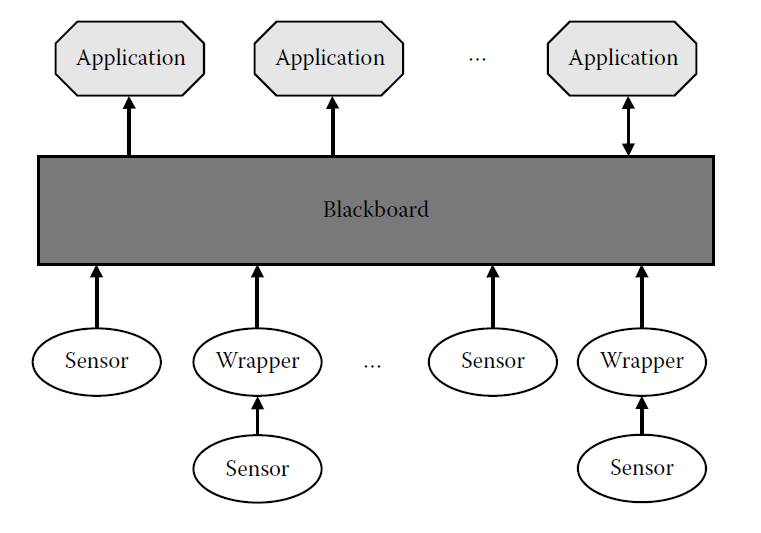
\includegraphics[scale=0.4]{images/blackboard}
\caption{Систем за развој на апликации со знаење за контекстот заснован на
школска табла (Blackboard)}
\label{fig:blackboard}
\end{figure}
 
Другиот спротивен пристап на пристапот со виџети е моделот на школска табла.
Темните табли (blackboards) имаат зачетоци од програмскиот јазик Linda и моделот
на простор на листи од парови во раните 1980ти [33]. Програмскиот јазик Linda
овозможува мал број функции за интеракција со глобален систем за перзистирање,
наречен простор на листа од парови (tuple space). Извршни компоненти може да
запишуваат, читаат или бришат информации во овој систем. Подоцна системите со
школска табла ја додаваат можноста да ги известуваат компонентите кога
информациите од интерес се додадени во таблата. Наспроти пристапот со виџети кај
кои барањата за информации се вршат директно врз компонентите преку механизам за
откривање, пристапот на школска табла овозможува барања за информации да доаѓаат
и се справуваат од единствен, централизиран простор на листи од парови. Воопшто,
контекст системите засновани на школска табла се едноставна имплементација на
традиционалните системи со темни табла, оптимизирани за перформанси и збогатени
со поддршка за XML енкодирање и декодирање на информациите.

И двата пристапи имаат свои предности и недостатоци. Пристапот на школска табла
е многу често неефикасен, особено кога количеството на податоци расте и
просторот на листи со парови се зголемува со што пребарувањето на одредени
парови станува многу тешко. Исто така, многу често овој систем е премногу силно
интегриран со апликацијата што предизвикува проблеми со синхронизацијата. Овој
проблем предизвикува задоцнување во модификација на апликацијата, конкретно во
просторот со податоци кој е ограничен поради тоа што не подржува комплексни
податочни структури. Моделот заснован на виџети исто така има доста проблеми од
аспект на робустност и конфигурација, со што тешко се справува со динамичката
природа на апликациите со знаење за контекстот, затоа што овие апликации имаат
потреба да се поврзуваат и исклучуваат од одредени компоненти како што
корисникот се движи, а неговиот контекст се менува.

Меѓутоа, овие два пристапи и не се меѓусебно исклучиви. Од перспектива на
развивач на инфраструктура, и за двата пристапи се потребни извори на контекст,
дали да се креираат виџетите или да се внесе контекстот во просторот со листи од
парови. Пристапот со контекст виџети овозможува добар модел за ефикасно
искористување на изворите на контекст, без разлика кој пристап се користи во
самата апликација. Од друга страна, моделот со школска табла овозможува
поедноставна апстракција на овие извори на контекст и го поедноставува
пренесувањето на контекстот до неговите консументи. Овој модел може да се
искористи во пристапот со виџети, каде на виџетите може да им се наложи да се
поврзат на некоја централизирана компонента (на пример, систем за откривање),
кој ќе одреди кој и каков ќе биде патот на контекстот од виџетот до консументот.
Од перспектива на развивач на апликации работата е многу олеснета со можноста да
се сокријат деталите на технологијата на сензорите и вчитувањето на контекстот
преку виџети. Нема потреба да се грижиме за индивидуалното поврзување на
компонентите во апликацијата со контекстот преку темни табли или контекст виџети
и механизмот за откривање.

\section{Проблеми во развојот на апликации со знаење за контекстот} 

Во овој дел се разработени аспектите на кои треба да им се посвети особено
внимание во развојот на апликациите со знаење за контекстот. 

\subsection{Контекстот како прокси за човечката намера}

Крајната цел на знаењето за контекстот е преку него да се дознае намерата на
корисникот. Апликациите ќе ја искористат оваа намера на човекот за соодветно да
се прилагодат преку обезбедување информации или преземање некакви акции.
Меѓутоа, информациите за контекстот се само прокси за оваа намера. Во
туристичките водичи во музеј, кога корисникот стои до одредена изложба може да
претставува дека корисникот има интерес кон неа, но може и да значи дека тој е
свртен со грб кон изложбата и разговара со пријател. Ваков е случајот во скоро
сите ситуации и апликации. Без разлика колку контекст може да се обработи во
апликацијата, секогаш е потребно повеќе за да се одреди вистинската намера на
корисникот. Кога се дизајнира апликација, развивачите мора да го дефинираат
опсегот на видови на ситуации кои апликацијата ќе ги препознава и разбира и
притоа помирувајќи се со фактот дека апликацијата може да направи неточно
прилагодување кон одредена ситуација кога таа ситуација е надвор од опсегот на
дизајнираната апликација. Апликацијата треба да искажува и некаква
веродостојност на нејзиното верување за одредена ситуација која е препознаена,
како што тоа го прави на пример системот со Активни Значки (слика 1). Ако
веродостојноста не е над некоја одредена граница, може да се побара и потврда од
корисникот пред да се изврши некоја акција, што е применето на пример во агентот
Clippy на Microsoft и во Lookout system [34].

\subsection{Препознавање на контекстот и проблеми во препознавањето}  

Системите со знаење за контекстот примаат некакви податоци на влез и одредуваат
и одлучуваат како ќе одговорат на овие податоци. Препознавање на контекстот е
делот во кој од податоците од сензорите треба да се добие разумен заклучок за
ситуацијата во која се наоѓа корисникот. Откако ќе се препознае ситуацијата на
корисникот, апликацијата може да преземе соодветна акција. Како што веќе е
споменато, скоро секогаш влезните податоци се недоволни да се препознае
соодветната ситуација, така да ова носи дополнителни проблеми од тоа како да се
разреши оваа несигурност во контекстот и улогата на правилата и машинското
учење.

Системите со знаење за контекстот имаат многу извори на недоследност, грешки или
тешкотии во препознавањето: сензорите како извори на контекстот може да работат
неточно, да откажат или да бидат несигурни во своите податоци; системите за
препознавање на контекстот може да бидат непрецизни или да носат неточни
заклучоци за одредена ситуација или бидат несигурни во своите заклучоци и
апликациите може да извршат неточни акции или да бидат несигурни која акција
треба да ја извршат. Повеќето системи со знаење за контекстот го сокриваат ова
или едноставно се однесуваат како да не постои. Една од важните одлуки за
дизајнерите која треба да ја донесат е дали да го моделираат контекстот со
можност за непрецизност или не. Однесување како да не постојат грешки и
непрецизности го поедноставува целиот процес на дизајн, но води кон не
флексибилни системи во однос на прецизноста на податоците. Спротивно, прифаќање
дека грешките и недостатоците постојат значи дека се моделираат системи кои
подобро го отсликуваат реалниот свет, но внесуваат и повеќе предизвици во
развојот и користењето. Грешката често се специфицира со некаков број кој
претставува веројатност или веродостојност на одредена вредност од контекстот.

Еден од пристапите за справување со непрецизноста на контекстот е да се
комбинираат повеќе различни извори за истиот вид контекст со цел да се подобри
прецизноста. Ова е познато како спојување (фузија) на сензори [35]. На пример,
при препознавање на активност, може да се искористи скриен Марков модел со
различни сензори и споените резултати да се репрезентираат како резултатна
матрица (confusion matrix) на множеството од можни активности [36]. Алтернативен
пристап е да им се овозможи на корисниците самите да ја разрешат несигурноста во
контекстот [37]. Наместо да се потпира целосно на автоматизиран процес, овој
пристап го користи знаењето на корисникот за ситуацијата да помогне во
разрешувањето на несигурноста во вчитаниот и одреден контекст. На корисникот
може да му се понуди листа од на пример N најдобри интерпретации на контекстот
со најголема веројатност и точност, а потоа да се побара да ја избере „точната“
интерпретација.

\subsection{Правила наспроти машинско учење}  

Апликациите со знаење за контекстот најчесто се дизајнираат со множество на
ако/тогаш правила: ако апликацијата препознае некоја одредена ситуација, тогаш
треба да изврши одредена акција. Правилата се создаваат едноставно, затоа што
целото знаење за секое од правилата е хомогено репрезентирано и овие системите
засновани на правила релативно лесно се развиваат затоа што постојат голем број
на постоечки под-системи кои одредуваат кога некое правило е задоволено.
Правилата се исто така доста интуитивни и едноставни за работа. Меѓутоа, овие
системи имаат и свои недостатоци: тие се склони кон создавање конфликти меѓу
правилата поради некоја скриена зависност, со што е прилично тешко кога треба да
се додаде некое ново правило, посебно кога бројот на правила е доста голем.
Едноставно тешко е да се следи текот на контролата меѓу правилата, а тие се исто
така и извор на не ефикасност, затоа што системот за одлучување преку правила
мора да ги измине сите правила за да одреди дали некое правило, ако воопшто, е
задоволено. Мали исклучоци кон некое правило може да значат дека тоа правило не
е исполнето или некое сосема друго правило е исполнето (она кое го претпочита
развивачот).

Познат алтернативен пристап е да се примени машинско учење. Наместо да се
создава листа на правила за тоа како апликацијата треба да се однесува,
развивачот на апликацијата може да собира податоци од видовите на ситуации со
кои се соочуваат корисниците и видовите на акции кои ги посакува. Потоа може да
се примени машинско учење да се научи веројатносната врска меѓу ситуациите и
акциите, наместо овие врски да се кодираат и бидат детерминистички. Ова сè уште
бара од апликацијата да овозможи инфраструктура и можности за прибирање на
контекстот и иницијално преведување на сензорските податоци во соодветната
ситуација. Машинско учење може да се примени и во врската меѓу сензорските
податоци и акциите, со што ќе се прескокне средниот чекор на идентификација на
контекстот. Недостатоците на овој пристап се што може да биде тешко да се научат
врските, а можно е и да е потребно големо количество податоци. Исто така ова се
прилично тешки методи за детектирање и отстранување грешки, а и не се интуитивни
за развивачот на апликацијата или крајниот корисник.

\subsection{Приватност}    

Системите со знаење за контекстот често имаат потреба да собираат големи
количества на лични информации за индивидуалците. Она што секогаш постои како
опасност при собирањето на вакви приватни податоци е можноста да се објават на
погрешни луѓе или во погрешни ситуации. Конкретно, затоа што овие системи
најчесто се дистрибуирани на повеќе компоненти и компјутерски мрежи, постои
реална можност да овие контекстни информации се дисиминираат несоодветно или пак
да се дисеминраат на компонента на која не може да и се верува. При развојот,
развивачите треба да обезбедат овие приватни информации да се споделуваат само
меѓу компонентите кои вистински имаат потреба да ги користат и споделуваат овие
информации. Исто така, развивачите треба да обезбедат да се зачувува приватноста
на корисникот и информациите да не се користат на несоодветен начин или на начин
за кој корисникот смета дека е несоодветен. Проблемот на приватноста е доста
комплексен и вообичаено се разработува посебно. Не постојат едноставни одговори
за тоа како да се обезбеди задоволителна приватност.

\subsection{Евалуација}    

Апликациите со знаење за контекстот, покрај многуте специфичности се одликуваат
и со својството дека се тешки за евалуација. Затоа што овие апликации се зависни
од контекстот, ретко може да се тестираат во лабораториска околина. Многу е
тешко да се симулира контекстот или ситуацијата од интерес. Дури и при
евалуација на терен, некои од овие ситуации се многу ретки така што голем е
предизвикот да се тестира и евалуира на различен аспект од квалитативен. Како да
се евалуираат овие апликации е исто така интересна тема за истражување и тема на
некои тековни истражувања [38][39][40].

\chapter{Мобилни социјални мрежи и сервиси}    

Мобилните социјални мрежи овозможуваат корисниците да бидат постојано поврзани
еден со друг, да споделуваат информации и со помош на мобилната технологија да
создаваат нови мобилни заедници. Со појавувањето на iPhone во 2007, земајќи ги
предвид хардверските и софтверските можности на овој уред се овозможи сонот на
многу корисници за вистински мобилни компјутери. Во овој дел се разгледуваат
мобилните социјални мрежи од нивните првични примери се до денешните современи
сервиси и се идентификуваат и категоризираат според соодветниот вид на податоци,
начин на работа и правила на приватност.

Со преку три милијарди корисници на мобилни телефони мобилната комуникација е
незаменлив дел во секојдневниот живот на луѓето во поголем дел од светот.
Широката распространетост на оваа технологија овозможи луѓето да се чувствуваат
постојано поврзани и достапни во секое време и на секоја локација. Во многу
истражувања се разгледувани ефектите од секојдневното користење на мобилни
телефони [41][42][43][44][45].

Постојат и мислења и истражување дека мобилните телефони може да доведат до
атомизација и оддалечување меѓу корисниците со тоа што ја намалуваат
комуникацијата лице во лице во урбани околини [46][47][48].

Како што напредува и самата мобилна технологија, се развиваат нови сервиси за
мобилни телефони кои овозможуваат корисниците да создаваат, развиваат и да ги
зајакнуваат социјални врски. Слично на сајтовите на социјалните мрежи на
интернет [49][50][51][52][53], мобилните сервиси може да им помогнат на
корисниците да изградат значајни мрежи за споделување информации и други ресурси
[54].

Еден од првите мобилни социјални уреди е Lovegety во Јапонија [55]. Lovegety е
самостоен уред кој може да се носи во дланка и испушта звук кога е во близина од
околу пет метри до некој друг сличен уред со исти карактеристики. Постојат уреди
како „розова девојка“ и „сино момче“ со три можности за прилагодување: ``let's
chat'', ``let's karaoke'' или ``get2''. Кога два вакви уреди се во близина еден
до друг и се слични прилагодувања  (на пример двата уреди се поставени на
``let's chat'') испуштаат звук и светат зелено. Ако се различно прилагодени
уредите звучно ќе сигнализираат и ќе светнат црвено. Според желбите на
корисникот, ако не сака да се поврзе и комуницира со друг корисник на Lovegety
може да се исклучи звукот, да се сокрие уредот или да се преправа дека не
поседува таков уред.

Постојат два вида информации кои се споделуваат со користење на Lovegety. Прво,
информација која се однесува на идентификација на луѓето кои се заинтересирани
да го користат мобилниот уред за да среќаваат други луѓе, второ, информации што
се однесуваат на тоа каков вид на социјална интеракција бара секоја од
личностите. Информациите кои се споделуваат се прилично едноставни, но
овозможуваат луѓето да имаат интеракција со непознати во јавни простори со помош
на посредување со мобилни уреди без да откриваат лични информации како број на
мобилен телефон или пак име.

MIT Media Lab и Intel Corporation развиле две од првите мобилни социјални мрежи.
Social Serpendity е Bluetooth базиран социјален сервис на MIT развиен со цел да
ја искористи моќта на мобилната технологија и социјалните информации [56].
Social Serpendity овозможува социјална интеракција меѓу корисници на географски
блиски локации преку пронаоѓање слични кориснички профили и споделување на
информациите од овие кориснички профили. Jabberworcky е сервисот на Intel кој се
обидува да го надгледува и известува за движењето на корисниците со цел да
идентификува т.н. „познати странци“ со што би се постигнало поголемо чувство за
урбана заедница [57]. Две од овие технологии се потпираат на мобилноста на
уредите да ги одредат информациите за локацијата со цел да постигнат социјални
врски меѓу корисниците.

Раните верзии на мобилните социјални сервиси, како што се Lovegety, Seredipity и
Jabberwocky, се најчесто развивани како самостојни апликации за мобилните уреди.
Но со напредокот на мобилните уреди, постои придвижување од одделни мобилни
уреди кои ја користат социјалната поврзаност кон мобилни социјални сервиси кои
работат на мобилни телефони. Мобилните телефони станаа дел од нештата без кои
луѓето не ги напуштаат своите домови како што се клучеви и паричници. Така,
повеќето од јавно достапните мобилни социјални сервиси се развиени со можност да
се користат од мобилните телефони. Во овој дел е направен преглед на мобилни
социјални сервиси, од првите примери се до денешните и идентификувани се и
категоризирани разни мобилни социјални мрежи и сервиси. 

\section{Мобилни социјални сервиси} 

Под мобилни социјални сервиси се подразбира софтвер, апликации или системи за
мобилни телефони кои овозможуваат корисниците да се поврзуваат со други луѓе,
споделуваат информации и создаваат нови технолошки напредни мобилни заедници. Се
користат многу различни термини за да се опишат овие видови на сервиси
вклучувајќи ги и следниве: мобилна социјална мрежа, мобилен социјален софтвер,
сервис на мобилна социјална мрежа или мобилен блог.

Терминот мобилна социјална мрежа еволуира од појавувањето и издигнувањето на
социјалните мрежни сервиси (SNS) како што се Facebook, MySpace и Friendster. Во
[51] се дефинираат сајтовите на социјалните мрежи како „веб-базирани сервиси кои
им овозможуваат на индивидуалците да (1) создадат јавен или делумно јавен профил
во рамките на затворен систем, (2) да создадат листа од други корисници со кои
тие споделуваат некоја врска и (3) да ја гледаат и изминуваат нивната листа на
врски и врските направени од други во самиот систем“. Нај-очигледната разлика
меѓу мобилните социјални мрежи и стандардните социјални мрежи е во тоа што овие
вторите се веб-базирани, а додека првите се примарно наменети за мобилни
телефони и мобилни корисници.

Со дефиницијата од [51] исто така се диференцирани мобилните социјални мрежи од
мобилниот социјален софтвер. Мобилните социјални мрежи овозможуваат на
корисниците да ги идентификуваат корисниците со кои се поврзани и да ги
прелистаат нивните врски во самиот систем. Понекогаш оваа навигација се прави
преку апликација на мобилниот телефон, а понекогаш на соодветниот веб-сајт на
кој се пристапува преку компјутер. Како што напредува самата мобилна
технологија, можноста да им се пристапува на овие информации преку мобилните
уреди се зголемува, со што голем број од овие сервиси ќе бидат целосно базирани
за мобилни телефони. Мобилниот социјален софтвер се разликува од мобилните
социјални мрежи во однос на тоа што тој вообичаено се инсталира на еден мобилен
уред (или е инсталиран уште пред да се купи уредот), додека мобилната социјална
мрежа не побарува специјална апликација или програма да се извршува на телефонот
со цел да работи. Понекогаш мобилните социјални мрежи се целосно базирани на
кратки текст пораки (СМС), сервисот за мултимедијални пораки (ММС) или пренос на
говор. Мобилниот социјален софтвер не е неопходно да ги исполнува овие услови
кои се идентификуваат во дефиницијата за социјални мрежи. Овој софтвер може да
нема артикулирана листа на социјални врски меѓу корисниците, туку неговата цел е
да овозможува некаков вид социјална интеракција меѓу веќе поврзаните мобилни
корисници. На пример, и Jabberwocky и Social Serendipity се класифицираат како
мобилен социјален софтвер, а не мобилни социјални мрежи, со тоа што и двете
овозможуваат социјална интеракција меѓу групи на мобилни корисници, но не
содржат и прикажуваат разни социјални врски меѓу корисниците.

Една од другите разлики кои може да се воочат е дека мобилниот социјален софтвер
овозможува помали или поголеми групи на мобилни корисници да споделат информации
меѓу себе во динамична околина при што тие може да се на иста или различни
локациии. Притоа овие корисници најчесто немаат претходни социјални врски при
што ваквото поврзување може да им помогне да се групираат за постигнување на
некоја заедничка цел. За разлика од ова, во социјалните мрежи како на пример
Facebook, повеќето од врските се базираат на претходни познанства и
пријателства. Слично и мобилните социјални мрежи пред сè овозможуваат поврзување
со луѓето со кои веќе се познаваме или имаме некои врски во надворешниот свет.
Притоа и самите маркетинг кампањи на повеќето мобилни социјални мрежи го
поттикнуваат поврзувањето на интернет со нашите постоечки пријатели без притоа
да форсираат создавања на нови пријателства и врски.

\section{Категоризација на мобилните социјални мрежи} 

Постојат огромен број нови мобилни социјални сервиси и сите од нив имаат некои
заеднички карактеристики но и разлики по кои може да се категоризираат. Со помош
на традиционалната топологија според медиумот за пренос [58], три фактори може
да се искористат да се категоризираат овие мобилни системи, а тоа се: медиумот
за пренос, начинот на комуникација и нивото на приватност.

Првиот фактор за категоризацијата на мобилните социјални мрежи е медиумот на кој
овие системи работат. Терминот медиум означува начин на комуникација, како што
се комуникација преку мобилен телефон, компјутер или безжичен уред. И покрај
сите трендови за конвергенција на технологиите, некои мобилни социјални мрежи
единствено се базираат на мобилните телефони како начин на поврзување меѓу
корисниците. Некои други безжични уреди користат Bluetooth за поврзување, а
повеќето мобилни социјални мрежи користат некаков вид на интернет базирани
врски. Често постои и некаква веб компонента на мобилната социјална мрежа со што
таа не е целосно базирана на мобилните телефони туку се интегрира и со веб
сервиси.

Со идентификување на одреден медиум кој се користи во различни мобилни социјални
мрежи, може да се направи поделба на самите системи. Исто така значајно да се
напомене дека медиумот во мобилните социјални мрежи го налага и пренесувањето на
пораки од еден на еден (меѓусебно) до еден на многу (повеќекратен пренос).
Мобилниот телефон најчесто укажува на  начин на комуникација меѓу двајца луѓе
преку текстуални пораки или говор. Можноста мобилната социјална мрежа да
пренесува информации на повеќе луѓе претставува значајно поместување во начините
на мобилната комуникација. Можноста за пренос на пораки на повеќе луѓе одеднаш е
важен фактор во мобилните социјални мрежи затоа што овозможува група на
корисници да комуницираат брзо и едноставно.

Вториот фактор по кој се категоризираат мобилните социјални мрежи е начинот на
комуникација. Начинот на комуникација се однесува на различните форми на
комуникација на кои членовите имаат можност да вршат интеракција едни со други,
вклучувајќи текст, слики, говор (или аудио) и видео. Мобилните социјални мрежи
се разликуваат меѓу себе според начините на комуникација кои ги овозможуваат, со
тоа што некои се ограничени на неколку, за разлика од други кои овозможуваат
многу повеќе начини. Начините на комуникација го обликуваат видот на интеракција
на корисниците во мобилните социјални мрежи. На пример, понекогаш постои
ограничување на бројот на знаци кои корисниците може да го испратат преку
мобилните социјални мрежи.Секој од овие модели го одредува обликот на
комуникација кој се случува во рамките на мобилната социјална мрежа.

Третиот фактор според кој се разликуваат мобилните социјални мрежи е нивото на
приватност. Мобилните социјални мрежи овозможуваат различни нивоа на приватност
според кои комуницираат нивните корисници со нивните социјални врски. Некои
системи ги прикажуваат одредени врски на корисниците, додека други мобилни
социјални мрежи прикажуваат профили на корисниците но не и врските со други. Ако
не се прикаже врска, системот ќе се класифицира како мобилен социјален сервис
или софтвер над мобилната социјална мрежа. Друг аспект од приватноста според кои
се разликуваат е дали системите овозможуваат заемни поврзувања или овозможуваат
еднонасочни врски. На пример, некои мобилни социјални мрежи овозможуваат
корисниците да испраќаат пораки до одредени луѓе, но да примаат од други луѓе.
Некои сервиси го нарекуваат ова гледање или следење. Корисник може да следи мала
група на луѓе, но може да биде следен од многу поголема група и обратно. На
пример, популарниот НБА кошаркар Шекил Онил, на социјалната мрежа Twitter го
следат 3,164,034 луѓе, а тој следи 614 луѓе. Систем со заемни врски не
овозможува пораки во еден правец. Во овие системи, корисниците испраќаат и
примаат пораки кон и од исти луѓе. Овие специфики на мобилната социјална мрежа
го диференцираат множеството од различни сервиси кои им помагаат на корисниците
да се поврзат со други корисници на основа на слични интереси или географска
блискост.

\begin{table}[!hbp]
\caption{Категоризација на мобилни социјални сервиси}
{\scriptsize{
\begin{tabular}{|p{.1\textwidth} | p{.2\textwidth} | p{.2\textwidth} |
p{.2\textwidth} | p{.2\textwidth}|}
\hline
 Име & Опис & Медиум & Начин на комуникација & Приватност\\
 \hline
 MySay & Зборувај му на вебот & Мобилен телефон, веб & Аудио (говор), текст, 
 слики, видео & Без јавно прикажување на социјалните врски\\
 \hline
  Cromple & Одржувајте ги информирани вашите пријатели со овој едноставен блог
  систем & Веб, мобилен телефон & Текст & Еднонасочни мрежи на пријатели\\
  \hline
  Jaiku & Вашиот разговор & Веб, мобилен телефон, IM & Текст, слики &
  Еднонасочни мрежи на пријатели\\
  \hline
  Pownce & Испраќај нешто на твоите пријатели & Мобилен, веб, IM & Текст, слики,
  видео, аудио & Еднонасочни мрежи на пријатели\\
  \hline
  Twitter & Што правиш? & Мобилен, веб, IM & Текст, слики & Еднонасочни мрежи на
  пријатели\\
  \hline
  Twitxr & Сликата вреди илјада зборови & Мобилен, веб & Слики, текст &
  Еднонасочни мрежи на пријатели\\
  \hline
  Utterz & Споделете ги вашите вести & Мобилен, веб & Слика, видео, аудио,
  текст & Еднонасочни мрежи на пријатели\\
  \hline
  Dodgeball & Поврзи се со твоите пријатели & Мобилен телефон, веб & Текст &
  Мрежи со взаемни пријателства\\
  \hline
  Facebook Mobile & Користи го Facebook во движење & Примарно мобилен телефон
  (додаток на Facebook.com) & Текст, слики & Мрежи со взаемни пријателства\\
  \hline
  Loopt & Претвори го твојот мобилен во социјален компас & Мобилен телефон
  (GPS), веб, IM & Текст, слика & Мрежи со взаемни пријателства\\
  \hline
  MySpace Mobile & Место за пријатели & Примарно мобилен телефон (додаток на
  MySpace.com) & Текст & Мрежи со взаемни пријателства\\
  \hline
  Radar & Разговори со слики со твоите омилени луѓе и никој друг & Мобилен, веб,
  IM & Слики, видео, текст, аудио & Мрежи со взаемни пријателства\\
  \hline
  Socialight & Откривај информации за местата околу тебе овде и сега & Мобилен
  телефон (GPS), веб & Слики, текст & Мрежи со взаемни пријателства\\
  \hline
\end{tabular}
}}
\label{tab:categorization_mobile_services}
\end{table}

Табела 2 ги категоризира следниве мобилни социјални сервиси според видот на
медиумот, начинот на комуникација и приватност: Powence.com, Twitxr, Twitter,
Jaiku, MySay, Utterz, Cromple, Facebook Mobile, MySpace Mobile, Dodgeball,
Socialight, Loopt, Kyte и Radar. Топологијата од [58], иако од 1973 се уште е од
голема помош во категоризацијата на овие сервиси. На пример, постојат значајни
разлики во начинот на комуникација. Првите мобилни социјални мрежи, како што е
Dodgeball, се примарно текст-базирани, а денешните сервиси постојано растат и
нудат повеќе модална комуникација. На корисниците им се нуди можност да
испраќаат текст, слики, аудио и видео. На пример, MySay и Utterz се обидуваат да
се диференцираат од другите мобилни социјални сервиси со тоа што дозволуваат
корисниците да го снимаат својот говор на нивните мобилни телефони и потоа да го
објават на веб.

Оваа категоризација на мрежите исто така ја прикажува и конвергенцијата на
медиумите за комуникација. Дизајнерите на мобилните социјални мрежи развиваат
специјални апликациски верзии на нивните сервиси, кои може да се интегрираат во
други веб сајтови како што се блогови или сајтови на социјални мрежи. На пример,
луѓето не мора веќе да одат на веб сајтот на Twitter за да се приклучат, туку
може директно да се поврзат од некој друг сајт на социјална мрежа како на пример
Facebook. Не само што овие сервиси овозможуваат повеќе начини на комуникација,
туку тие исто така овозможуваат и пренос на поголем број на различни видови
податоци. Покрај севкупната конвергенција која се случува во однос на медиумите
за пренос и видовите на податоци кои се пренесуваат, сепак сè уште најголеми
мобилни социјални сервиси се оние кои произлегуваат од популарните социјални
мрежи на веб. И покрај тоа, овие сервиси се уште не се развиени како вистински
мобилен софтвер и не ја искористуваат мобилноста и контекстот на корисниците,
туку се само додаток на нивните веб сајтови наменети за мобилни уреди.

Може да се постави и прашањето дали терминот мобилни социјални мрежи е
вистинскиот начин да се опишат ваквите социјални мрежни сервиси кои овозможуваат
пристап до различни видови на податоци од социјалната мрежа на повеќе различни
технолошки платформи? И покрај конвергенцијата на сите видови на податоци,
мобилната социјална мрежа е термин кој се уште е од помош бидејќи ја потенцира
мобилноста, индивидуалноста и пристапот на системи кои се наменети за мобилни
уреди. Мобилните телефони се дефинирани преку нивната мобилност. Тие не се
врзани за кујната, канцеларијата или телефонската говорница, туку може да се
најдат на секакви различни простори. За разлика од фиксните линии, мобилните
телефони примарно се врзани за одредена личност. Луѓето најчесто поседуваат
нивни лични мобилни телефони, додека приватните фиксни линии се вообичаено
врзани за одредено место. Пристапноста, индивидуалноста и мобилноста на
мобилните телефони е она што ги прави посебно моќни комуникациски технологии и
ги прави различни од традиционалните компјутерски технологии.

\chapter{Дизајн и архитектура на системот} 

Во претходните два дела беа опишани две различни области кои се основа во
дизајнот и архитектурата на мобилни апликации со знаење за контекстот. Во делот
за пресметување со знаење за контекстот дефиниран е контекстот, опишани се
категориите на различни видови апликации со знаење за контекстот. Притоа опишани
се и неколку софтверски шаблони и рамки по кои треба да се водиме во развојот и
архитектурата на мобилна апликација која сакаме да користи контекстуални
информации. Мобилните социјални мрежи и сервиси се област која во последните
години претрпува огромен развој и трансформации и има огромна улога во
архитектурата и развојот на денешните мобилни апликации. Преку интеграција на
мобилната апликација со овие мрежи и сервиси се обезбедува еден многу значаен
елемент од контекстот на корисниците на мобилната апликација, како што се
неговите пријатели, лични контакти и други социјални врски. Преку овие
информации може да се дознае повеќе и за личните интереси на самиот корисник со
што самата апликација се доближува едно ниво поблиску до корисниците
овозможувајќи високо ниво на персонализација во сервисите кои ги нуди.

\section{Гео Настани} 

Гео Настани е прототип систем преку кој се обидуваме да ги презентираме
опишаните концепти на дизајн и архитектура на апликација со знаење за
контекстот. Системот Гео Настани е замислен како интеграција на веб-сервер,
мобилни клиенти и мобилни социјални мрежи со што се постигнува еден вид мобилен
веб-сервис за организација и промовирање на приватни и јавни настани. Под настан
подразбираме некое случување од каков било вид кое се случува во одредено време,
на одредена локација и е наменето за собирање на група луѓе за одредена цел со
што се постигнува некаков вид на социјализација. Настанот се организира на тој
начин што одреден корисник или повеќе корисници објавуваат јавно или на нивни
пријатели за местото, времето и целта за нивно заедничко собирање и извршување
на групна социјална активност. Денес постојат неколку веб-сервиси кои
овозможуваат организирање и управување на настани како што се Upcoming [59] на
кој себеси се опишуваат како календар на настани, додека Eventful [60] е друг
веб сервис кој им помага на корисниците да пребаруваат, следат и споделуваат
информации за настани. Исто така еден од најпопуларните начини за креирање и
споделување информации за настани е тој што го нуди веб сајтот на социјалната
мрежа Facebook [61] и претежно е наменет за неформални настани организирани и
наменети за сопствениот круг на пријатели. Речиси сите вакви сервиси
овозможуваат креирање, пребарување, споделување информации за приватни или јавни
настани, а некои од нив имаат и мобилни компоненти за кој овозможуваат одредени
функционалности. Во некои од нив се обработува и локацијата на корисникот со што
може да се сметаат и за еден вид на локациски базирани сервиси. Ниту еден од
овие системи не го разработува или вклучува знаењето за контекстот на
корисниците. Во ваков вид на системи, ова знаење може многу да се искористи и да
помогне во подобрување на самите сервиси и генерално подобрување на корисничкото
искуство. Она што системот Гео Настани го поседува во својата архитектура е
мобилната компонента која претставува мобилна апликација што го собира
контекстот на корисникот, соодветно го обработува и извлеченото знаење го
користи да понуди подобар и персонализиран сервис. Притоа оваа мобилна
апликација се интегрира преку еден вид сервисно ориентирана архитектура со
серверската компонента, а се интегрира и со мобилните социјални мрежи со што се
постигнува еден вид модуларна архитектура во кој секоја компонента е независна и
може да биде заменета со друга.

Системот е составен од клиентска мобилна компонента, веб-сервер компонента и
некоја мобилна социјална мрежа. Мобилната компонента е мобилна апликација која
го следи моделот на модуларен дизајн на апликација со знаење за контекстот
сличен на дизајнот со виџети. Серверската компонента од системот ги опслужува
барањата на мобилните клиенти и претставува централно место за интеграција на
мобилната апликација, мобилната социјална мрежа и основен репозиториум на сите
корисници на системот.

\begin{figure}[htb]
\centering
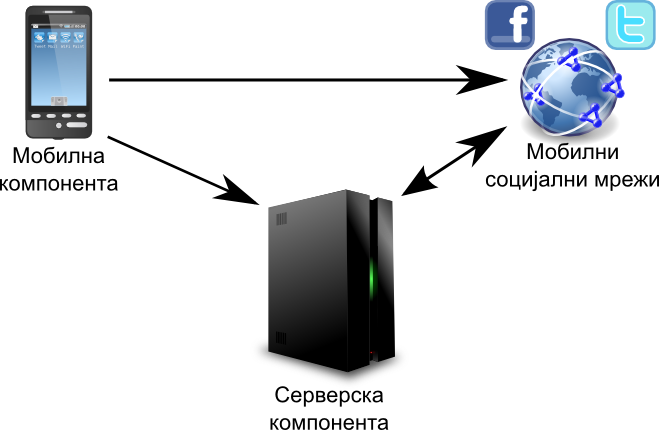
\includegraphics[scale=0.4]{images/architecture}
\caption{Глобална архитектура на Гео Настани}
\label{fig:architecture}
\end{figure}

 
Во центарот на оваа архитектура прикажана на слика 4 е серверската компонента
која ги обединува мобилната компонента и мобилните социјални мрежи. Оваа
компонента е основен дел во сервисно ориентираната архитектура (SOA) и
претставува множество на повеќе REST веб-сервиси кои ги обезбедуваат сите
функционалности кои се потребни во систем за организација на настани. Преку
множеството на веб-сервиси се овозможува креирање на корисници, настани,
пребарување по клучни зборови, локација и се останато што е потребно за
организација на настани од каков било вид. Она што е специфично во оваа
архитектура е што серверската компонента може да се замени со кој било
веб-сервис сличен на погоре споменатите кој обезбедува интерфејс за програмирање
(API) и ги нуди повеќето од можностите потребни за управување со информациите за
настаните.

\begin{figure}[htb]
\centering
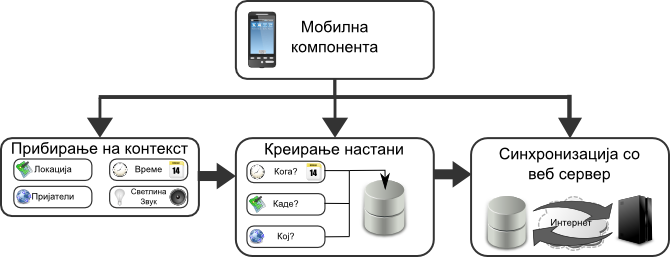
\includegraphics[scale=0.4]{images/mobile_component}
\caption{Архитектура на мобилната компонента на Гео Настани}
\label{fig:mobile_component}
\end{figure}
 
\section{Мобилна компонента}

Мобилната компонента на системот за организација на настани преставува клиентска
мобилна апликација која ги обединува активностите како што се прибирањето на
контекстот, креирањето на настани и синхронизацијата со веб серверот. На
\ref{fig:mobile_component} е прикажана архитектурата на мобилната компонента.
Таа е поделена на три посебни модули: модул за прибирање на контекстот, модул за
креирање настани и модул за синхронизација со веб серверот.

\begin{figure}[htb]
\centering
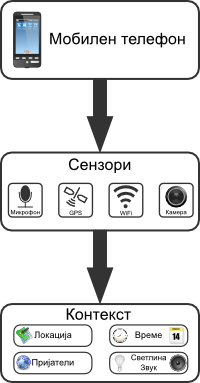
\includegraphics[scale=0.4]{images/context_aquisition}
\caption{Собирање на контекстот во мобилната апликација}
\label{fig:context_aquisition}
\end{figure}

 
Собирањето на контекст е една од најважните компоненти во архитектурата на
мобилна апликација со знаење за контекстот. Во оваа компонента со помош на
користење на соодветни сензори и дополнителни уреди
(\ref{fig:context_aquisition}) се восприемаат информации за контекстот,
соодветно се моделираат и се пренесуваат до релевантните делови од мобилната
апликација.

Следејќи го процесот на развој на апликации со знаење за контекстот прибирањето
на контекстот се одвива со следните неколку чекори: 
\begin{itemize}
  \item Спецификација - во оваа фаза
според доменот на апликација ги извојуваме локацијата, времето, пријателите како
контекст кој треба да се преземе и искористи во апликацијата.
  \item Преземање - за оваа фаза се развиени неколку модули кои ги користат
  соодветните интерфејси за пристап до соодветните сензори и ги преземаат
  потребните информации за конкретниот елемент од контекстот. На пример, за
  локацијата како дел од контекстот тоа може да се моментната локација преку
  латитуда и лонгитуда добиени од интегрираниот GPS уред.
  \item   Испорака и прием - во оваа фаза се моделираат информациите од контекстот и се
  испорачуваат до оние делови во апликацијата за кои се релевантни овие
  информации. За таа цел во модулите од претходната фаза се
моделира контекстот и се обезбедува интерфејс за пристап.
\item Акција - во оваа фаза апликацијата извршува дел од своите предвидени акции но со
дополнително знаење за контекстот преку обработка на информациите примени во
претходната фаза. Со тоа акциите кои се извршуваат се разликуваат во начинот на
извршување предизвикано од самиот контекст.   
\end{itemize}

Креирањето на настани е фазата во која корисникот ги надополнува информациите за
контекстот во кој се наоѓа со цел да се дојде до доволно информации за креирање
на ентитет настан. Ова дополнување на информации означува едноставно додавање на
информации како име на настанот, поместување на времето на настанот или пак може
да биде и модифицирање на некои информации за контекстот како локацијата преку
дополнително опишување. Бидејќи се работи за мобилна апликација наменета за
мобилни уреди, а самите мобилни уреди ги сметаме за доста лични уреди, голема е
веројатноста за одредување на идентитетот на корисникот, односно идентификување
на корисникот со сопственикот на тој мобилен уред. Користејќи го овој значаен
дел од контекстот во фазата на креирање на настани се користи и социјалниот дел
од контекстот составен од листата на контакти која ја поседува самиот корисник.
Откако ќе му се понуди оваа листа со контакти, тој може да изврши дополнително
потпомогнато експлицитно збогатување на контекстот со листа на контакти кои се
поканети на настанот кој го креира, ако се работи за приватен настан.

Во фазата на синхронизација со серверот се одвива целокупната комуникација на
мобилната компонента со серверската компонента во системот. Оваа фаза може да се
извршува на неколку начини и е значајна од неколку аспекти. Нејзиното извршување
може да биде автоматски поттикнато од одредени настани во апликацијата без
знаење на корисникот, а може да се иницира и со конкретна акција за
синхронизација од самиот корисник. Автоматското иницирање се случува кај акции
како креирање на нов настан со цел синхронизација и запазување на интегритетот
на податоците, а се случува и при секое ново стартување на апликацијата со цел
да се започне користење на истата со целосно синхронизирани и ажурирани
податоци. Исто така автоматско иницирање може да се случи и како резултат на
промена на контекстот. Конкретно се работи за дел од контекстот поврзан со
состојбата на поврзаност на мобилниот уред за некоја мобилна мрежа, односно дали
мобилниот телефон има отворена врска со некоја мобилна мрежа и има пристап на
интернет или не е поврзан на мобилна мрежа и не може воопшто да извршува акции
поврзани со синхронизација со серверот. Ако е во состојба на поврзаност акцијата
за синхронизација може автоматски да се стартува.

\section{Одредување на локацијата на корисникот} 

Можноста да се одреди локацијата на корисникот овозможува многу мобилни
апликации да ги прилагодат своите функционалности и сервиси на соодветната
локација и контекст. Знаењето на локацијата на корисникот овозможува апликациите
да им дадат многу поголема точност, а со тоа и вредност на своите сервиси. Денес
луѓето користат локациски базирани апликации во речиси сите сегменти од животот,
како што се забава, навигација, следење на предмети, следење на здравствената
состојба како одговори на ургентни повици и др. Бројот на апликации со знаење на
локацијата на корисникот е во огромен пораст, а се повеќе овие апликации се
развиваат за денешните паметни телефони искористувајќи ги нивните можности за
позиционирање пред сè преку вградените GPS уреди.

Локацијата е еден од најважните елементи на контекстот на корисникот [12].
Покрај тоа што информацијата за локацијата е корисна сама за себе таа може да се
искористи и за одредување на дополнителни информации за контекстот на корисникот
како неговата активност, начинот на транспорт или социјалните врски. На пример,
ако сме повеќе време во сала за вежбање тоа е јасна индикација дека извршуваме
некоја активност поврзана со вежбање, додека ако се движиме со брзина од 90 км/ч
е показател дека се возиме со некое превозно средство.

Информациите за локацијата може да се претстават во апсолутна, релативна или
симболичка форма. Апсолутна локација претставува точна позиција како адреса или
географски координати. Пример, ФЕИТ се наоѓа на ул. „Руѓер Бошковиќ“ б.б.
Релативна локација опишува некоја локација во однос на некоја друга апсолутна
локација. Пример, ФЕИТ се наоѓа околу 3 км западно од Владата на РМ. Симболичка
локација е некое описно име за некоја позната локација како на пример „дома“,
„на работа“ или „во кујна“ и сл. Во повеќето мобилни апликации може да се
користат сите од овие форми на локација, меѓутоа со најголема вредност за
повеќето е апсолутната локација и таа е една од нај-користените форми.

И покрај важноста на информациите за локацијата, сè уште не постои некоја
унифицирана технологија што е прецизна, доволно евтина, лесна за имплементација
и широко распространета. Наместо тоа, постојат колекција од технологии за
лоцирање, при што секоја од нив е за одредена намена, со различни прецизности
која се движи во границите од 1 милиметар со користење на магнетни полиња до
десетици километри со користење на ФМ радио сигнали. Со оглед на тоа што
технологиите за лоцирање се некаков компромис меѓу прецизност и цена, треба да
се избере систем за лоцирање кој ги задоволува потребите на соодветната
апликација. Кај апликациите за мобилни телефони тоа значи дека се избира некоја
од овозможените технологии кои ги нуди самиот телефон или пак се прави
комбинација од сите методи кои ги нуди со помош на некаков софтвер.

\subsection{Карактеристики на технологиите за лоцирање} 

Технологија за лоцирање е комбинација на методи и техники за откривање на
физичката локација на објект или личност во реалниот свет. Локацијата е позиција
во физичкиот простор и како што видовме може да се претстави во апсолутна,
релативна или симболичка форма.

\subsection{Репрезентација на локација} 

Најчестата форма на претставување на прецизна
апсолутна локација е со користење на степените на латитудата и лонгитудата на
точката на површината на Земјата, како што е дефинирано со географскиот
координатен систем. Ако ја земеме Земјата за перфектен елипсоид, со латитудата
се мери аголот меѓу точката и екваторијалната рамнина од центарот на Земјата. Во
реалноста, латитудата, или геодетската латитуда, го мери аголот меѓу екваторот и
линијата која е нормална на референтниот елипсоид, кој ја апроксимира формата на
Земјата. Со лонгитудата го мери аголот меѓу Екваторот и дадената точка. Линијата
која поминува во близина на Кралската обсерваторија, Гринич, Англија, е
прифатена како нулта лонгитуда и е наречена примарен меридијан. Линиите со
константна латитуда се наречени паралели, а линиите со константна лонгитуда се
наречени меридијани. Меридијаните, за разлика од паралелите, не се паралелни и
сите се сечат на Северниот и Јужниот пол. Оваа форма на репрезентација на
локацијата често се користи во локациските системи за отворен простор како што е
GPS. 

Локацијата на Земјата може да се означи и со користење на латитуда и лонгитуда.
На пример, Скопје, Р. Македонија, има латитуда 42\textdegree01$'$ N и лонгитуда
21\textdegree26$'$E. Така, вектор од центарот на Земјата до точката
42\textdegree01$'$ северно од екваторот и 21\textdegree 26$'$ источно од Гринич,
Англија, ќе помине низ Скопје. Со додавање на вертикалното растојание од
центарот на Земјата, или најчесто од средната вредност на нивото на морето на
дадена точка, можно е да се специфицира било која локација под или над
површината на Земјата. Иако географските координати се корисен начин за
определување прецизна апсолутна локација, тие не се соодветни за користење во
апликации кои вклучуваат читање на локациски информации од страна на луѓето.
Ретко може да се случи некој да разбере човек кој би рекол: „Се наоѓам на
30.5432 Север, 65.2344 Запад, или пак дали сакаш да пиеме кафе на 30.552 Север,
64.934 Запад за половина час?“. Како алтернатива, најчесто се користи адреса за
означување локација (на пример, Ул. Маршал Тито 37), симболичко име за местото
познато на двајцата учесници во разговорот (пр. трговскиот центар) или релативни
координати (на пример, 50 метри јужно од мостот). Сервиси за гео-кодирање може
да претвораат адреси и поштенски кодови во географски координати, додека
преведувањето географски координати во адреса или поштенски код може да се
направи со користење на спротивен геокодер. Многу поголем е предизвикот на
одредување локација во затворени простории. Системот може да ја претставува
локацијата во зградата со користење на X и Y растојанијата од одредена фиксна
точка или агол во зградата, додека во зграда со повеќе катови референтна точка
може да се постави на секој кат. Иако ваквиот начин на репрезентација може да е
корисен за системот, сепак вака репрезентираните локации вообичаено се
поврзуваат со концепти на повисоко ниво на симболичка репрезентација, како
„дневна соба“, „спална“, „канцеларија“ или „до автоматот за кафе“.

\begin{figure}[htb]
\centering
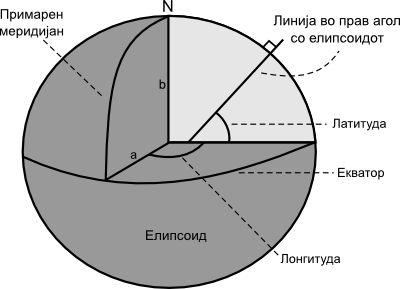
\includegraphics[scale=0.4]{images/gps_coordinates}
\caption{Пример латитуда и лонгитуда на точка на Земјата}
\label{fig:gps_coordinates}
\end{figure}

 
\subsection{Инфраструктура и клиентски базирани системи за лоцирање} 

Генерално постојат три системи за лоцирање: клиентски базирани, мрежно базирани
и мрежно потпомогнати. Во клиентски базиран систем за лоцирање, уредот ја
пресметува сопствената локација без да се потпира на мрежната инфраструктура.
Пример за клиентски базиран систем за лоцирање е GPS, во кој уред опремен со GPS
чип ја пресметува сопствената локација со користење на сигнали кои се примаат од
барем четири GPS сателити.

Во
мрежно базиран систем за лоцирање, мрежната инфраструктура ја пресметува
позицијата на уредот. Пример за мрежно базиран систем за лоцирање е системот
Активна значка [12] во кој значката која ја носат корисниците емитира
инфрацрвени (IR) сигнали кои се примаат од инфрацрвени примачи поставени на
плафонот. Потоа, примачите ги пренесуваат податоците за сигналите до мрежен
процесор кој ја пресметува локацијата на значката. 

Кај мрежно потпомогнатите
системи за лоцирање, и уредот и инфраструктурата учествуваат во пресметувањето
на локацијата на уредот. Пример за мрежно потпомогнат систем за лоцирање е
потпомогнат GPS (A-GPS), во кој уредот ја пресметува сопствената локација врз
база на сопствените GPS мерења и дополнителни информации за констелацијата на
GPS кој се примаат преку линк од мобилната мрежна инфраструктура. Дополнителните
информации му овозможуваат на уредот да ја пресмета сопствената локација и во
недостиг на четири сателити во видното поле и со тоа го намалува времето
потребно за добивање на првата локација. 

Основните предности на клиентски
базиран систем за лоцирање е тоа што ја задржува приватноста на локацијата на
самиот уред. Со тоа што самиот со помош на податоци од инфраструктурата ја
пресметува својата локација без да пренесува податоци, инфраструктурата нема
начин да ја одреди локацијата на уредот, освен ако самиот уред не ги сподели тие
податоци. Од друга страна, пресметување на локацијата на уредот ја троши
батеријата и додава дополнителни барања за пресметковна моќ и големина на
меморија на самиот уред. 

\subsection{Техники за одредување на локацијата} 

Во овој дел се
опишани шест основни техники за одредување на локацијата на уредот: блискост,
трилатерација, хиперболичка трилатерација, триангулација, земање примероци и
пресметување на слепо. Во некои од овие техники се претпоставува претходно
знаење на референтни точки, чија прецизна локација е позната однапред. Примери
за референтни точки се GPS сателит, Wi-Fi пристапна точка (AP) или базна
станица.

\subsubsection{Блискост}  
 
 Чувствувањето на оддалеченоста е нај едноставна техника за
лоцирање. Се користи близината на уредот до референтна точка за да се пресмета
локацијата на уредот. За локација на уредот вообичаено се зема локацијата на
референтната точка. И уредот и референтната точка може да ја чувствуваат
оддалеченоста. Откривање дека некој уред е во близина не имплицира дека се
открива и идентитетот на тој уред, така што за да се открие идентитетот потребен
е посебен механизам. 

Близината може да се открие преку директен физички контакт
или ако уредот се постави во опсегот на една или повеќе референтни точки. На
пример, чекорење врз сензор за притисок означува нечие присуство, а исто така и
комуникација со Wi-Fi пристапна точка означува близина на некој уред до таа
пристапна точка. Во вториот случај, чувствувањето на близината е врз база на
ограничен опсег на покривање на безжичната технологија. На пример, опсегот на
комуникационен уред со мало поле е неколку сантиметри, опсегот на Bluetooth уред
е десетици метри, опсегот на Wi-Fi уред е стотици метри, додека мобилен телефон
може да прима сигнали од базна станица која е оддалечена со километри. Ако
уредот се наоѓа во границите на повеќе референтни точки, можно е да се пресмета
поточна локација. На пример, можно е да се пресмета локацијата на уредот како
просек од позициите на референтните точки. Ако е достапна силината на сигналот
со кој референтните точки го слушаат уредот, може да се пресмета уште по точна
локација со воведување тежини на просеците на референтните точки. 

\subsubsection{Трилатерација}

Трилатерација е техника за лоцирање која ја пресметува позицијата на уредот
преку мерење на растојанијата меѓу уредот и неколку референтни точки на познати
позиции. Бројот на референтни точки потребен за пресметување на локацијата е за
еден поголем од физичката димензија на просторот. На пример, за пресметување на
локација на уред во дводимензионален простор (2-D) потребни се 3 неколинеарни
референтни точки, додека за пресметување на локација во 3-D потребни се четири
референтни точки. 

\begin{figure}[htb]
\centering
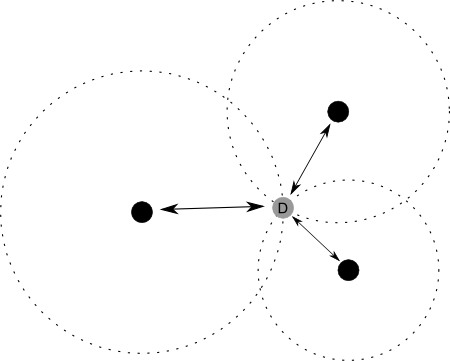
\includegraphics[scale=0.4]{images/trilateration}
\caption{Пример трилатерација во 2-Д. Црните точки претставуваат референтни
точки додека сивата точка е локацијата на уредот.}
\label{fig:trilateration}
\end{figure}

На \ref{fig:trilateration} е прикажана трилатерација во 2-Д. Секоја од црните
точки претставува референтна точка и го дефинира центарот на кругот со радиус
еднаков на пресметаната оддалеченост на уредот. Така, пресметување на
оддалеченоста од една референтна точка дава неограничен број на можни локации на
уредот на периметарот на кружницата. Пресметување на две должини до две
референтни точки дава две можни локации на уредот на пресечните точки на двете
кружници, додека пресметување на три референтни точки единствено ја дефинира
локацијата на уредот. За да се пресмета растојанието меѓу уредот и референтна
точка, често се мери или времето потребно за пристигнување на сигналот или се
мери ослабувањето на силината на сигналот во примачот.
 


\subsubsection{Хиперболичка латерација}

Хиперболичката латерација ја користи разликата на времињата на пристигнување на
сигналите од уредот до три или повеќе референтни точки, наместо да го користи
самото време на патување на сигналот. Техниката на хиперболичка латерација може
да се користи кога уредот прима сигнали кои се симултано испратени од три или
повеќе референтни точки. Во продолжение ќе биде објаснета 2-Д хиперболичка
латерација. Сигналот испратен од уред ќе се прими во различни времиња од
референтни точки на различни позиции на различно растојание од уредот. Разликата
меѓу времињата на пристигнување на сигналот испратен од уредот до две референтни
точки ја ограничува можната локација на уредот на хипербола, при што двете
референтни точки се фокусни точки на хиперболата. На слика 9 е прикажана
хиперболичка латерација во две димензии. Пресекот на двете хиперболи уникатно ја
означува локацијата на уредот.

\begin{figure}[htb]
\centering
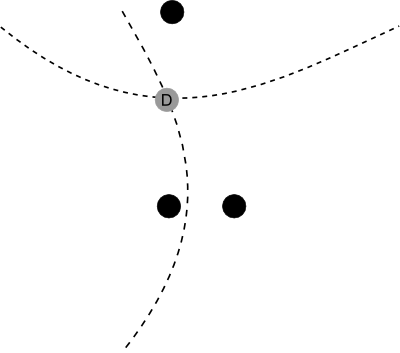
\includegraphics[scale=0.4]{images/trilateration_h}
\caption{Пример хиперболичка латерација во 2-Д. Црните точки претставуваат референтни точки, а сивата точка е локацијата на
уредот.}
\label{fig:trilateration_h}
\end{figure}
 
\begin{figure}[htb]
\centering
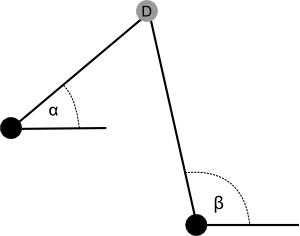
\includegraphics[scale=0.4]{images/triangulation}
\caption{Пример за триангулација во 2-Д. Црните точки претставуваат референтни
точки, а сивата точка е локацијата на уредот.}
\label{fig:triangulation}
\end{figure}

\subsubsection{Триангулација}

 За да се пресмета локацијата на уредот кај триангулацијата се
користи аголот на пристигнување (AOA) на сигналите кој потекнуваат од уредот а
се насочени кон референтните точки. На слика 10 е даден пример на триангулација
во 2-Д. Со мерење на аголот со кој сигналот пристигнува од уредот (преставен со
сива точка) до референтните точки (претставени со црни точки) ја ограничува
позицијата на уредот на линијата која поминува низ референтната точка под аголот
на пристигнување. Мерење на аглите од две референтни точки резултира со две
линии кои уникатно ја дефинираат локацијата на уредот во точката на пресек.
Така, доволно е да се има мерења од само две референтни точки за да се одреди
локацијата на уредот во две димензии, иако често во практиката се користат
повеќе од две референтни точки за да се намалат грешките при мерење. 
За да се
пресмета аголот на пристигнување на сигналот, се користи или насочена антена или
низа од антени. Бидејќи ниту едната ниту другата не се вообичаени за мобилен
уред, најчесто се користат мерењата на референтните точки, кои вообичаено
претставуваат базни станици. 

\subsubsection{Земање примероци} 

Земањето примероци е техника за
локација која користи техники од препознавање на облици за да се пресмета
локацијата на уредот. Иако земањето примероци може да се изведе од многу
различни сензори како што се за звук, светлина и слично, сепак овде ќе го
објасниме со земање примероци на радио сигнали. 

Земањето примероци на радио
сигналите е базирано на две својства на радио сигналите: временска стабилност и
просторна варијабилност. Временска стабилност се однесува на стабилноста на
радио сигналот од одреден радио извор на било која локација во текот на времето.
Јачината на сигналот на одредена локација во тек на времето зависи од јачината
со која сигналот се зрачи од предавателот (која вообичаено е константна) и
апсорпцијата на сигналот од средината (воздух, ѕидови или други препреки).
Просторната варијабилност се однесува на променливоста на радио сигналот од
истиот извор на две различни локации. На пример, силината на сигналот од
непосредната базна станица е различен во канцеларијата и во кафетеријата.
Системите за лоцирање ја земаат предноста на овие две својства преку запишување
на радио профилите на различни физички локации и користење на овие профили за
подоцна да се одреди локацијата. 

Прецизноста на системот за земање примероци е
тесно поврзан со степенот на просторна варијабилност на самиот сигнал. На
пример, силината сигналот од Wi-Fi пристапна точка покажува просторна
варијабилност од 1 до 10 метри, или со други зборови, дадена пристапна точка
може да се слуша посилно или воопшто да не се слуша на неколку метри
оддалеченост. Ова овозможува систем базиран на земање примероци од Wi-Fi
пристапни точки да има околу 1m просторна грешка. 

Многу значајно во земањето
примероци е фазата на тренинг со цел да се изгради радио мапа на целната околина
пред да може да се користи за одредување на локацијата. Во тек на фазата за
тренинг, уредот се движи низ околината, и ја мери силината на сигналот кој се
емитира од група на радио извори (на пример, Wi-Fi пристапни точки). Пример на
радио мерења е даден во Табела 3. Во табелата е прикажана листа со Wi-Fi
пристапни точки и силината на сигналот примен од секоја од пристапните точки.

\begin{table}[!hbp]
\caption{Пример на мерења во кои е вклучено името (SSID), MAC адресата и
силината на сигналот (RSS) од три Wi-Fi пристапни точки}
\begin{tabular}{|p{.3\textwidth} | p{.3\textwidth} | p{.3\textwidth}|}
\hline
SSID (Име) & BSSID (MAC Адреса) & Силина на сигналот (RSS)\\
\hline
ETF WLAN CSD & 00:0e:6a:d3:16:35 & -70\\
\hline
M.F. & 00:23:69:e3:55:e8 & -89\\
\hline
DIPteam & 00:1e:e5:5b:5e:22 & -93\\
\hline
\end{tabular}
\label{tab:samples}
\end{table}

На крајот на фазата за тренинг, системот за земање примероци има радио профил на
повеќе локации во одреден физички простор. Поради тоа што земањето примероци не
ја моделира пропагацијата на радио бранови, прилично густа мрежа на мерења треба
да се собере за да се постигне добра прецизност. Во еден од оригиналните системи
за земање примероци [62], на пример мерењата на силината на сигналот од Wi-Fi се
вршени на 1m оддалеченост. 

Откако ќе заврши фазата со тренинг, уредот може да ја
пресмета сопствената локација со едно мерење и пренесување на резултатите на
системот за земање примероци, кој може да се наоѓа на самиот уреди или на некој
сервер во мрежата. Системот за земање примероци ја пресметува локацијата на
уредот преку пресметување на сличност меѓу моменталните мерења и мерењата
запишани во фазата на тренинг. 

Сличноста меѓу мерењата може да се пресмета на
повеќе начини, меѓутоа често се користи Евклидово растојание во просторот на
сигналите. На пример, ако едно Wi-Fi мерење содржи јачина на сигнали за N
пристапни точки $(S_1, \ldots ,S_n)$ и друго мерење ги содржи мерењата на
јачините на сигналите од истите $N$ извори $(R_1, \ldots ,R_n)$, Евклидовото
растојание меѓу двете мерења се пресметува како:\\
\[
    E = \sqrt{(S_1 - R_1)^2 + \ldots + (S_n - R_n)^2}
\] 

Ако некоја
пристапна точка не е присутна во едно од мерењата, често се заменува јачината на
нејзиниот сигнал или со минималниот сигнал во мерењето или со фиксна
предодредена вредност. 

Постојат повеќе варијации на алгоритмот за земање
примероци. Систем за земање примероци, базиран на алгоритмот за најблизок сосед
$(NN)$ ја пресметува локацијата на уредот како локацијата во мерењата од тренинг
радио профилот со најмало Евклидово растојание од моменталното мерење. Додека со
$k-NN$ алгоритмот се пресметува локацијата на уредот со усреднување на локациите
на $k$ мерења во тренинг профилот со најмалото Евклидово растојание од
моменталното мерење. Идеалното $k$ може да се одреди преку експеримент во
соодветна репрезентативна околина, но мали вредности од 3 до 4 се покажуваат
добро во практика [63].
 
\begin{figure}[htb]
\centering
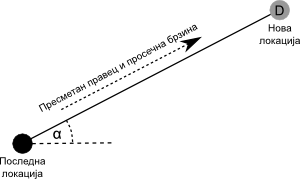
\includegraphics[scale=0.4]{images/dead_reconing}
\caption{Пример на слепо пресметување во 2-Д. Црната точка претставува последно
добиената локација, а сивата претставува пресметаната нова локација.}
\label{fig:dead_reconing}
\end{figure}
 
\subsubsection{Слепо пресметување}

Слепо пресметување е техника за лоцирање која
ја пресметува локацијата на уред на основа неговата претходна локација која е позната,
изминато време од моментот кога е добиена локацијата, правецот и просечната
брзина на движење. Претпоставката  во позадина на слепото пресметување е дека
правецот и просечната брзина на движење од последно добиената локација се или
познати или може да се пронајдат. На \ref{fig:dead_reconing} е илустриран принципот на
слепото пресметување. Црната точка ја претставува последно позната локација на уредот.
Со знаење на овој податок, правецот и просечната брзина, можно е да се пресмета
новата локација на уредот претставена со сивата точка. 

Ограничувањето на ваквото
пресметување е што ја пресметува релативната позиција од последно добиената
локација, така да мора да се користи во комбинација со други технологии за
лоцирање кои имаат можност да ја пресметаат апсолутната локација на уредот.
Слепото пресметување често се користи да се подобрат пресметките од некој друг
систем за лоцирање или да ја пронајдат локацијата кога другиот систем не е
достапен (на пример, кога автомобил влегува во тунел и го губи сигналот од GPS
сателитите). 

Прецизноста на слепото пресметување зависи од квалитетот на
пресметките за брзината и правецот на движење како и прецизноста со која е
одредена почетната локација. Овие вредности може да се добијат преку
екстраполација од две претходни локации или преку мерења од некои сензори на
самиот уред. Некои од сензорите кои често се користат при слепо пресметување се
акцелерометри, кои можат да го измерат забрзувањето на уредот, одометри, кои го
пресметуваат растојанието поминато со автомобил или жироскопи, кои се користат
да го пресметаат правецот на движење. 

\subsection{Можни грешки во одредувањето локација}

Целта на системите за лоцирање е да дадат точна информација за локацијата на
одреден уред, а со тоа и локацијата на корисникот. За жал, во практика,
системите за локација често произведуваат неточни информации поради различни
причини.

\subsubsection{Извори на грешки} 

Системите за лоцирање се дизајнирани да даваат што е можно
поточни информации за локацијата ако мерењата кои ги врши системот се исто така
точни. Сепак, постојат неколку фактори кои воведуваат грешки во системите за
лоцирање. 

\emph{Неточни координати на референтните точки.} Системите за лоцирање на кои
им е потребна прецизна локација на референтните точки продуцираат грешки кога
соодветните локации не се точни. Проблемот може да се избегне или да се реши со
внимателно мапирање на референтните точки. Меѓутоа, за некои референтни точки
кои се мобилни (на пример, GPS сателити) ова може да биде тежок проблем поради
некои неочекувани фактори (на пример, соларни ветрови) кои може да ја променат
локацијата на референтната точка. 

\emph{Јоносферично и тропосферично задоцнување.} Сигналите кои патуваат преку
јоносферата и тропосферата трпат одредени задоцнувања како резултат на интеракциите со атмосферата на Земјата. Иако
постојат математички модели кои се обидуваат да го пресметаат ова задоцнување,
тоа сè уште е причина во поголемиот дел на грешки во GPS базираното
позиционирање. 

\emph{Синхронизација на времињата.} Прецизно мерење на времето побарува
многу прецизна синхронизација меѓу времињата на испраќачот и примачот на
сигналот или меѓу уредите кои испраќаат сигнали истовремено. Постојат алгоритми
за синхронизација кои го намалуваат ефектот на не синхронизирани времиња, но не
ги отстрануваат целосно. Изместувањата на времињата се чести извори на грешки
кај сите системи за лоцирање кои ги користат мерењата на времињата за одредување
на локацијата. 

\emph{Повеќе патишта.} Сигналот кој патува низ просторот може да
пристигне на целната локација преку повеќе различни патишта поради интеракцијата
со пречките на кои може да наиде. Копии на сигналот може да интерферираат пред
да бидат примени од примачот и притоа да имаат дисторзирана амплитуда и фаза.
Ако се нема видлива линија од испраќачот до примачот, проблемите со повеќе
патишта се посериозни и предизвикуваат поголеми грешки во мерењето. 

\emph{Геометрија.} Геометриската конфигурација на референтните точки има голем
ефект на прецизноста. Позиционирање на референтните точки премногу блиску една до друга
или на иста линија вообичаено предизвикува големи грешки во локацијата.

Квалитетот на пресметаната локација која се добива од системот за лоцирање
зависи од повеќе фактори, вклучувајќи ја физичката локација, времето од денот,
моменталните временски околности и атмосферски влијанија како и самата околина.
Така, за целосно да се согледа квалитетот на еден систем за лоцирање, неопходно
е да се соберат голем број на пресметувања на локацијата за разни временски
услови. Процедурата за препознавање на грешките зависи од тоа дали системот
продуцира симболички или апсолутни локации. 

Локациските системи кои симболички
локации, како што се „на работа“ или „дома“, продуцираат резултати кои се или
точни или неточни. Во овој случај, нај често прецизноста се искажува преку
проценти. На пример, систем за лоцирање може да ја погодува собата во некоја
зграда 85\% од времето. Повторување на експериментот повеќе пати овозможува да
се пресмета ниво на доверба на прецизноста на системот. 

Кај системите за лоцирање
кои даваат апсолутни локации, како што се географски координати, вообичаено е да
се прикаже функција на распределба на кумулативна грешка. Во овој случај,
грешката во локацијата е дефинирана како растојанието меѓу вистинската и
пресметаната локација. Исто така често се искажува како 50\% или 95\% грешка во
лоцирањето, кои може да се извадат од функцијата на распределба на кумулативната
грешка. Ако системот работи различно во хоризонтална и вертикална димензија,
тогаш често и грешката се пресметува за секоја димензија. 

\subsubsection{Одредување на локацијата во Гео Настани} 

Како што претходно споменавме денешните
мобилни уреди се опремени со повеќето стандардни системи за лоцирање на корисниците како што е
лоцирање со помош на GPS, лоцирање со триангулација од базни станици, а можно е
и развивање на дополнителни системи за лоцирање. Локацијата несомнено е еден од
најважните елементи од контекстот кој се користи во Гео Настани. Барањата околу
прецизноста на локацијата која го сочинува контекстот на корисникот ја
исполнуваат сите системи за лоцирање достапни во паметните мобилни телефони.
Системот побарува локација во апсолутна форма со незадолжителна информација и за
симболичната форма. Форматот на информацијата за локацијата е латитуда,
лонгитуда и адреса или симболично име на локацијата. Она што е недостаток е
сложеноста на процесот на добивање на локација, затоа што тој зависи од многу
услови во кој корисникот бара да му се одреди локацијата. Сосема се разликува
начинот на одредување локација во отворен и затворен простор. Иако е општо
познато сепак многу малку корисници знаат дека добивање на GPS прецизна локација
во затворен простор е речиси невозможно, или дека добивањето на првичната
локација со помош на триангулација е многу побрзо отколку со GPS системот.
Затоа, во архитектурата на Гео Настани дополнително е развиена компонента за
полесно и интуитивно одредување на локацијата на корисникот. 

Во основа овој
подсистем е комбинација од понудените системи за лоцирање во мобилните телефони,
збогатени со контекстни информации внесени експлицитно од корисникот, како и
постојана можност за избирање на сопствената локација на географска мапа или од
листа од претходно пресметани локации. Исто така додаден е модул за попрецизно
лоцирање во затворени простории кои е базиран на земање примероци од пристапните
точки на постојната Wi-Fi инфраструктура.

\begin{figure}[htb]
\centering
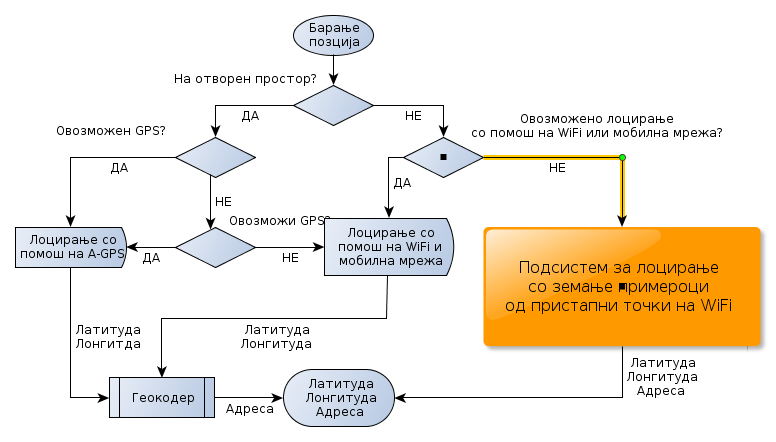
\includegraphics[scale=0.4]{images/locating_flow}
\caption{Дијаграм на активности на процесот на лоцирање на корисникот во
системот Гео Настани.}
\label{fig:locating_flow}
\end{figure}
 
На \ref{fig:locating_flow} е прикажан дијаграмот на активности на модулот
за лоцирање на корисникот во рамките на системот Гео Настани. 

\section{Серверска компонента} 

Серверската компонента е централниот дел во сервисно
ориентираната архитектура (SOA) според која се базира архитектурата на целиот систем. Сервисно
ориентирана архитектура во повеќето случаи се однесува на множество на
веб-сервиси имплементирани преку SOAP или XML-RPC стандардите со цел
комуникација и интеграција на повеќе различни клиенти со еден или повеќе
веб-сервери кои може да се наоѓаат на иста но и на повеќе различни локации. Ако
се погледнат денешните современи веб-системи кои на некој начин имплементираат
сервисно ориентирана архитектура, тоа го прават на малку поинаков начин. Причина
за избегнувањето на SOAP и XML-RPC стандардите е што тие се прилично комплексни
и бараат поголемо познавање на самите протоколи и програмските јазици за нивна
имплементација. Најголемиот дел од популарните веб сервиси своите
функционалности ги прават достапни преку објавување на множество на веб сервиси,
што во програмерскиот свет е по познато како API (интерфејс за програмирање
апликации).

\begin{figure}[htb]
\centering
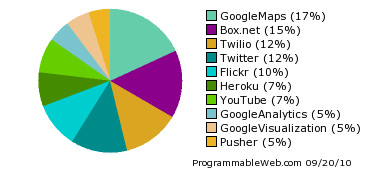
\includegraphics[scale=0.4]{images/web-services}
\caption{Листа на 10 нај користени API достапни на веб}
\label{fig:web-services}
\end{figure}

На \ref{fig:web-services} е дадена листа од нај
користените веб-сервиси на интернет достапни преку соодветно API\footnote{извор
http://www.programmableweb.com/apis}. Кај повеќето
од овие веб-сервиси се следи REST архитектурниот стил со што овој стил на
архитектура во софтверското инженерство е нај застапен во сервисно ориентираните
архитектури на интернет. 

Архитектурата на серверската компонента во Гео Настани
ги следи токму принципите на REST архитектурата. 

Архитектура на REST веб-сервиси REST [64] претставува архитектурен стил за дистрибуиран мрежен систем за
пренесување на ресурси од каков било вид. Во центарот на оваа архитектура се
ресурсите. Сите информации достапни на веб се некаков вид на ресурс. Тоа може да
бидат текстуални информации, слики или каков било друг вид на информации.
Клиентите може да пристапат на овие ресурси преку соодветното URL:
\\[.5cm]
\texttt{http://www.geoevents.mk/event/4321}
\\[.5cm]
по што резултатот што се добива е некаква репрезентација (representation) на
соодветниот ресурс (пр. HTML страница). Оваа репрезентација ја поставува
клиентската апликација во некаква состојба (state). Резултатот од пристапот до
некој друг хиперлинк на HTML страницата ја пренесува клиентската апликација во
друга состојба. Така клиентската апликација ја менува (transfers) состојбата со
секоја различна репрезентација на ресурсот. Според објаснувањето на авторот на
REST „целта е да се добие слика како добро дизајнираните веб апликации се
однесуваат: мрежа од веб страници (виртуелен дискретен автомат), каде
корисниците се движат низ апликацијата преку следење на линкови (транзиција на
состојби), со што како резултат се добива (репрезентација на следната состојба
на апликацијата) следна страница од веб апликацијата“.

\begin{figure}[htb]
\centering
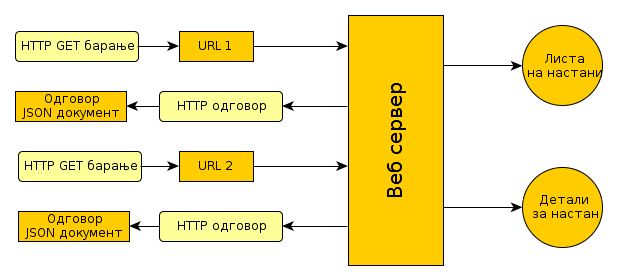
\includegraphics[scale=0.4]{images/rest_architecture}
\caption{REST архитектурен стил на дизајн на веб сервиси}
\label{fig:rest_architecture}
\end{figure}
 
REST претставува стил
на архитектура, а не стандард. Со тоа што не е стандард, не постои никаква
спецификација од некое тело за стандардизирање како W3C или некоја комерцијална
имплементација. Секој кој го следи стилот на оваа архитектура може да ги развие
своите сервиси на REST начин. Всушност многу имплементации на веб-сервиси се
всушност REST без самите да се свесни за тоа. 

Иако REST не е стандард, сепак корисни многу стандарди како:
\begin{itemize}
  \item HTTP
  \item URL
  \item XML/HTML/GIF/JPEG итн (репрезентација на ресурси)
  \item text/xml, text/html, application/json, image/gif, image/jpeg, итн (MIME
видови) 
\end{itemize}
 
Сите ресурси во REST се претставени со некакви логички URL, а секој
ресурс е некаков концептуален ентитет. Репрезентацијата претставува конкретна
манифестација на ресурсот. URL адресата:
\\[.5cm]
\texttt{http://www.geoevents.mk/events/3425}
\\[.5cm]

претставува логичко URL, кое се разликува од физичките URL. Така, може, но не
мора да постои статичка HTML страница за секој настан. Постоење на милиони
настани и милиони статички HTML страници за истите не е атрактивен дизајн.
Самите URL адреси не треба да откриваат никакви детали за техниката на
имплементација која се користи. Треба да имаме можност за менување на
имплементацијата без тоа да се одразува на клиентите или пак да се отстранат не
постоечки URL адреси. 

Некои од позначајните карактеристики на REST веб сервисите се: 
\begin{itemize}
  \item Клиент-сервер - интеракција со повлекување на ресурси (компонентите консументи
консумираат репрезентации на ресурси)
\item Без состојба - секое барање од клиентот до серверот мора да ги содржи сите информации потребни да се разбере
барањето и не може да се земе предвид контекстот на самиот сервер.
\item Кеширање - се зголемува ефикасноста на одговорите, но мора да постои
можноста соодветните ресурси да може да се означуваат дали имаат можност за кеширање или немаат.
\item Стандарден интерфејс – на сите ресурси им се пристапува преку генерички
интерфејс (на пример, HTTP GET, POST, PUT, DELETE)
\item Именувани ресурси - системот
се состои од ресурси кои се именувани со помош на соодветни URL.
\item  Меѓусебно
поврзани репрезентации на ресурси - репрезентациите на ресурсите се поврзани со
користење на URL, така што се овозможува клиентските апликации да ја менуваат
состојбата од една во друга.
\item Слоевити компоненти - медијатори, како што се
прокси сервери, сервери за кеширање, итн, може да се постават меѓу клиентите и
ресурсите за да се зголемат перформансите, сигурноста и сл.
\end{itemize}

Некои од позначајните принципи кои треба да се следат во дизајнот на REST
веб-сервиси се следните:
\begin{enumerate}
  \item Клучот во креирање на успешни веб сервиси во REST мрежа (како што е вебот) е
    да се идентификуваат сите концептуални ентитети кои сакаме да ги објавиме
    преку соодветни сервиси. Примери за такви ентитети во Гео Настани се: листа
    на настани, детали за настанот, место на одвивање на настанот.
    \item Создавање URL за секој ресурс. Ресурсите треба да се именки, а не глаголи. На
пример, лоша практика е да се користи:\\
 \texttt{http://www.geoevents.mk/events/getEvent?id=3425}\\ наместо глаголот
\texttt{getEvent}, треба да се користи именка:
\\\texttt{http://www.geoevents.mk/events/3425}\\
\item Категоризација на
ресурсите во однос на тоа дали клиентите може само да примаат репрезентација на
ресурсите или може да ги менуваат (додаваат нови) ресурси. За оние ресурси кои
може само да се читаат, треба да се овозможи пристап преку HTTP GET, додека за
ресурсите кои може да се менуваат треба да се овозможи HTTP POST, PUT, DELETE.
\item Пристапувањето на ресурси со HTTP GET не треба да предизвикува никакви странични
ефекти. Тоа значи, ресурсот треба само да врати репрезентација на ресурсот.
Повикување на ресурсот не треба да резултира во каква било модификација на ресурсот.
\item  Никој од ресурсите не е остров сам за себе. Со други зборови, треба да
се постават соодветни хиперлинкови во репрезентацијата на ресурсите за да се
овозможи клиентите да преземаат повеќе информации или да дојдат до некои слични
и поврзани информации. 
\item Дизајнирање со цел да се откриваат податоците постепено.
Не треба да се откриваат сите информации во единствен одговор на барањето. Треба
да се овозможат линкови за да се откријат повеќе детали. 
\item Спецификација на форматот на одговорот преку соодветна шема (DTD, W3C
Scheme, RelaxNG или Schematron). За оние сервиси за кои е потребно POST или PUT барање, треба да се
специфицира форматот на барањето. 
\item Опис како треба да се повикуваат сервисите или
преку WSDL документ или преку HTML документ.
\end{enumerate}
    
\subsection{Интеграција со социјални сервиси}

Со големата експанзија на социјалните мрежи, денес речиси и да не постојат луѓе,
пред се од технолошката ера кои не се присутни на некоја социјална мрежа.
Ваквата популарност доведува до огромно количество информации кое може да се
искористи во развојот на апликации. Социјалните мрежи се огромен извор на лични
контекстни информации како што се име, слика, информации за контакт, пол,
љубовен статус, интереси, активности, хоби, музички и филмски вкусови,
припадност на одредени групи и секако информации за поврзаност или пријателство
со други луѓе. Исто така, социјалните мрежи овозможуваат споделување на овие
информации со други корисници, со цел пронаоѓање на луѓе со слични интереси и
нормално воспоставување комуникации со тие луѓе. На социјалните мрежи може да се
гледа како на следниот чекор во природната еволуција на интернет, каде првиот
чекор беше можноста на луѓето да пристапуваат до информации (пример се милијарди
веб-страници со различни информации достапни до секого). За втор чекор во
еволуцијата може да се смета можноста за интеракција на корисниците со веб
сајтовите(пример се можностите за купување производи, создавање лични содржини и
нивно објавување). Следниот значаен и природен чекор е фокусиран на
остварувањето на комуникацијата на луѓето на интернет, а тука несомнено голем
бран предизвикаа многуте социјални мрежи кои успеаја да ги поврзат луѓето и да
им овозможат едноставни можности за директна комуникација и лесно споделување
информации и ресурси.

Интеграцијата на Гео Настани со социјалните мрежи е мотивирана од идејата дека
интегрирањето и прикажувањето на богатството од контекстуални информации од социјалните мрежи во
светот на реална комуникација на корисниците значително може да ја подобри
социјалната интеракција. Да разгледаме едно реално сценарио од системот Гео
Настани. Нека некој корисник присуствува на некој настан од социјален карактер
во кој има можност да остварува комуникација со останатите присутни на тој
настан. Ако во овој случај, на корисникот му се прикажат информации од јавните
социјални профили на другите присутни на настанот, а притоа системот ги
идентификува оние со слични интереси како неговите тој може лесно да ги пронајде
оние корисници со кои би сакал да оствари некој интересен разговор. Ако на
почеток кога го дефиниравме контекстот и рековме дека се тоа информации кои
луѓето ги знаат и лесно ги споделуваат во меѓусебна интеракција, а дека овие
информации потешко се спроведуваат во интеракцијата на луѓето со компјутерите,
сега имаме сосема спротивна ситуација, односно меѓусебната интеракција меѓу
луѓето ја збогатуваме со дигитални контекстни информации од социјалните мрежи на
веб.

\begin{figure}[htb]
\centering
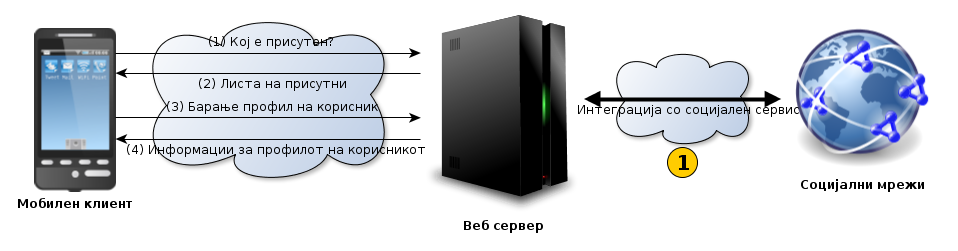
\includegraphics[scale=0.4]{images/social_context_1}
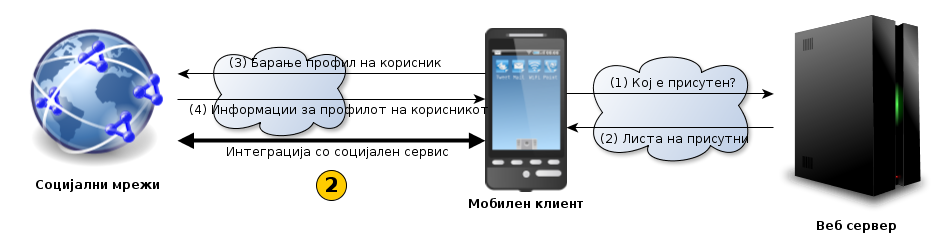
\includegraphics[scale=0.4]{images/social_context_2}
\caption{Две можни точки на интеграција со социјални сервиси во архитектурата
на Гео Настани}
\label{fig:social}
\end{figure}
 

За да се овозможи предложената интеграција во архитектурата на
мобилната апликација и веб серверот потребно е да се пронајдат точките на
интеграција на овие компоненти со социјалните сервиси. На \ref{fig:social} се
прикажани две можни точки на интеграција за конкретното сценарио кога се присуствува на
некој настан. Интеграцијата со социјалните сервиси може да се прави на веб
серверот, но може да се направи и од мобилните клиенти. 

Во првиот случај сите барања за информации поврзани со интеграција со
социјалните сервиси мобилниот клиент ги праќа до веб-серверот на апликацијата,
при што интеграцијата со социјалните сервиси се случува на серверот. Добрата
страна на овој пристап е што на веб-серверот може да се направи кеширање на
податоците од социјалните сервиси и тие не мора да се повикуваат на секое барање
на мобилниот клиент.

Во вториот случај точката на интеграција со социјалните веб-сервиси може да биде
на мобилниот клиент, при што тој ги извршува стандардните барања до веб-серверот
на апликацијата, меѓутоа кога е потребно да се повлечат информации од некој
социјален веб-сервис тоа се прави директно од мобилниот клиент.

Освен предложеното сценарио за интеграција на Гео Настани со социјални
веб-сервиси, можни се и други начини на интеграција со постоечки и популарни
социјални веб сервиси. Интеграцијата се прави за да се овозможат неколку
можности кои додаваат значителен социјален момент во мобилната апликација.
Конкретно преку интеграција се овозможуваат следниве значајни можности:
\begin{itemize}
  \item Споделување на содржини (настани, локации)
  \item Поврзување со корисници на други сервиси
  \item Групирање во групи и заедници со слични и заеднички интереси
  \item Можности за директна комуникација
\end{itemize}
    
  

\chapter{Имплементација и евалуација} 

Во овој дел се опишани имплементациските детали за мобилната апликација,
веб-серверот и компонентите за интеграција со социјалните сервиси. Прототипот на мобилната апликација е развиен за
оперативниот систем Android преку користење на Android SDK кој го користи
програмскиот јазик Java. Веб-серверот е развиен со користење на рамката за
развој на веб апликации Django во програмскиот јазик Python. Целокупниот развој
е направен на преносен компјутер Lenovo ThinkPad Т400 на оперативниот систем
Ubuntu 10.04, а како околина за развој е користен Eclipse IDE. Исто така
направено е тестирање и евалуацијата на мобилната апликација и целиот систем со
користење на два мобилни уреди од производителот HTC (HTC Hero, HTC Tatoo). 

\section{Имплементација на мобилната апликација}
Следејќи ја кратката спецификација и предложената архитектура и дизајн на
мобилната компонента од системот Гео Настани во имплементациската фаза се
имплементирани следните основни кориснички барања: 
\begin{itemize}
  \item Креирање на настани
  \item Прикажување настани во околината на
корисникот
  \item Прикажување настани за кои покажале интерес контактите и
пријателите на корисникот 
  \item Пребарување настани 
  \item Означување на присуство
на некој настан 
\end{itemize}
Од овие основни кориснички барања произлегуваат и други подетални
барања кои се однесуваат претежно на собирање информации за корисничкиот
контекст како локација, пријатели и податоци од други сензори. Овие барање се:

\begin{itemize}
  \item Одредување на локацијата на корисникот
  \item Поврзување со неговите контакти и
пријатели  
\end{itemize}


Слика 16. 

Разделување на основната мобилна апликација од компонентите за
собирање на контекстот на корисникот Основните барања на системот се
имплементирани преку една основна мобилната апликација, додека за дополнителните
барања кои произлегуваат од овие основни барања а се однесуваат на контекстот на
корисникот се имплементирани како посебни компоненти (апликации) кои преку
механизмите на оперативниот систем Android се интегрираат со основната
апликација. 

За собирање на контекстот на корисникот апликацијата користат две
посебни компоненти: компонентата која се користи како извор на локацијата и
компонентата која се користи како извор за социјален контекст на корисникот,
односно поврзување со неговите пријатели

 Слика 16. 
 
 Мобилната апликација
претставува клиент на REST веб-сервиси и повеќето од имплементациските детали се
однесуваат на најдобриот начин на имплементација на ваква апликација. Пред да
започнеме со деталите околу имплементацијата може да го поставиме прашањето
зошто би развивале посебна мобилна апликација како клиент на REST веб-сервисите,
кога најчесто овие сервиси имаат свои веб-базирани апликации кои може да се
извршуваат на мобилен веб прелистувач, а со тоа и на многу од современите
мобилни уреди. Како одговор на ова прашање постојат барем пет причини со кои би
го поткрепиле изборот за развивање на посебна клиент апликација: 1.  Интеграција
со платформата на мобилниот уред. Ова означува искористување на сите можности
кои ги нуди оперативниот систем на мобилниот уред и соодветните интерфејси за
програмирање. Ова вклучува пристап до сензорите, камерата, изворите на локација
и многу други сервиси на кои не може да им се пристапи од веб прелистувач. 2. 
Во случајот на Android платформата мобилната апликација може да се интегрира со
оперативниот систем на начин со кој ќе нуди сервиси и содржина на други
апликации преку механизам кој го обезбедува самиот оперативен систем. 3. 
Апликацијата може да се извршува во позадина. Операции за кои е потребно повеќе
време (како преземање на поголеми количества податоци од веб) може да се
извршуваат во позадина. Мобилните уреди ја губат поврзаноста со мрежата, така да
апликацијата може повремено во позадина да проверува кога повторно ќе биде
воспоставена врска со веб серверот и го искористи тоа за да ги обнови
податоците. 4.  Апликацијата е многу побрза од мобилната веб апликација. Во
клиент апликација може да се имплементира кеширање на податоците кои се
преземаат од веб. Исто така се врши трансфер на помало количество податоци (само
чистите податоци во некој стандарден формат како JSON или XML) за разлика од
повлекување на овие податоци во веб апликација заедно со соодветниот HTML и
JavaScript код. 5.  Мобилната апликација може да биде конзистентна со
оперативниот систем во поглед на корисничкиот интерфејс. Овозможени се и многу
можности за иновација во корисничкиот интерфејс и креирање подобро корисничко
искуство. Секако ако на корисниците им се понуди клиентска мобилна апликација
наспроти веб апликација повеќето ќе ја изберат мобилната апликација.
 
Слика 17. Едноставна имплементација на REST клиент На Слика 17 е прикажана еден
начин на имплементација на REST клиент. На прв поглед оваа имплементација
изгледа како вистинскиот и нај едноставен начин за имплементација на ваква
апликација. Само ако на проблемот на имплементација на REST пристапиме преку
детално согледување на повеќе можни имплементации може да дојдеме до подобро
решение. Во оваа имплементација која е прилично интуитивна имплементацијата на
REST клиент може да се идентификуваат пет фази. Во првата фаза активноста која е
основната градбена единка на мобилната апликација има потреба од пристап до
некој веб-сервис и го избираа соодветниот REST метод кој го исполнува барањето.
Барањето може да биде да се земат листата на настани, да се земат детали за
некој настан или било кој метод кој е достапен преку REST веб сервисите на веб
серверот. Во вториот чекор се извршува барањето до серверот, односно се
остварува повикувањето на веб сервисот преку HTTP протоколот. Ова барање
искористување на еден од методите кои ги нуди HTTP протоколот GET (за преземање
ресурси), POST (за креирање нови ресурси), PUT (за менување ресурси) и DELETE
(за бришење ресурси). Во овој чекор се случува комуникацијата со оддалечениот
сервер и се користат комуникациските можности на телефонот како Wi-Fi или
GPRS/EDGE. Третиот чекор е обработка на податоците кои се добиени како резултат
на HTTP барањето. Во овој чекор најчесто се врши трансформација на податоците од
форматот во кој се пренесуваат податоците (JSON, XML) во објектен модел со кој
се работи во самата апликација. Во следниот четврти чекор овие податоци се
складираат во некоја податочна структура која ги чува во работната меморија и од
каде може да се прикажат на корисничкиот интерфејс или да се прави било каква
друга манипулација со нив. Последниот чекор е оној во кој податоците се
зачувуваат од работната меморија во постојана меморија. Ова е процесот на т.н.
кеширање со што ако има потреба повторно да се прикажат истите овие податоци тие
може да се пристапат од локалната меморија наместо повторно да се прави барање
до веб серверот и да се повторува целиот овој процес. Оваа постапка значително
го забрзува пристапот до податоците кои се преземени претходно. Еден од
недостатоците на овој пристап е тоа што ако се прекине извршувањето на
активноста, што не е невозможно туку напротив често се случува, ресурсите ќе се
најдат во недефинирана состојба. Во имплементацијата на оперативниот систем
Android активноста како видлива компонента од извршувањето на некоја апликација
може да биде прекината во случаи кога се извршува во позадина. Во корисничките
сценарија на мобилниот телефон не е редок случај некоја активност да се постави
во позадина и да биде заменета со поприоритетни активности како одговарање на
телефонски повик или читање кратка текстуална порака. За да се избегне овој
недостаток потребно е операцијата како што е преземањето податоци од веб
серверот и нивната обработка да се извршува на начин на кој нема да може да биде
прекината од оперативниот систем во било кој момент. Во имплементацијата за
Android ова го овозможуваат сервисите. Секоја од активностите може да стартува
сервис во кој ќе имплементира функционалност за која е од значење да не биде
прекината, а може да трае подолго време.
 
Слика 18. Имплементација на REST методи со сервис На Слика 18 е дадена една
можна имплементација на REST метод со користење на сервиси. Во оваа
имплементација значајно е користењето на сервис за операцијата која се извршува
подолго време, а исто така значајно е што апликацијата постојано има информација
за состојбата во која се наоѓаат ресурсите кои се пренесуваат преку HTTP барања.
Во првиот чекор активноста врши иницијализација на помошна класа која се
справува со стартување на сервисот и повратните резултати. Во вториот чекор се
врши стартување на сервисот и поставување на соодветните повратни функции.
Процесорот е компонентата која ја врши обработката на податоците пред да бидат
испратени до серверот, а исто така е задолжен и за конзистентноста на состојбата
на ресурсите кои се разменуваат. Конкретно во четвртиот чекор се запишува
информација за состојбата на ресурсот пред тој да се побара од веб серверот или
пак се испрати на веб серверот. Оваа информација во секое време може да ни ја
даде состојбата на секој ресурс со што и корисникот може да биде соодветно
информиран за состојбата на податоците во апликацијата. Во петтиот чекор се
извршуваат соодветните HTTP барања до веб серверот. Во овој чекор се извршуваат
операциите чие време на извршување е подолго поради комуникацијата со
оддалечениот сервер. Времето на извршување во голема мера зависи од брзината на
трансфер кој може да се постигне со комуникациските можности на мобилниот уред.
Исто така во овој чекор може да се случи да се прекине целиот овој процес на
повикување на REST методите ако мобилниот уред ја изгуби врската. Откако во
седмиот чекор ќе се извести процесорот за извршувањето на HTTP барањето кон
соодветниот REST метод, во следниот осми чекор се менува состојбата на ресурсот
во локалната база на податоци. Во овој чекор сите компоненти на корисничкиот
интерфејс кои ги прикажуваат овие податоци се освежуваат со новите податоци. Во
последните неколку чекори се врши едноставно пропагирање на резултатот до
активноста иницијатор на извршувањето на REST методот. Ваквата имплементација на
клиент апликација за REST методи не е единствената и најдобра имплементација, не
една од неколкуте можни кои ги исполнува правилата за надежна и стабилна
имплементација.

\section{Имплементација на серверот} 
 
 Беб-сервисите од архитектурниот
стил REST кој беше изложен во архитектурата се интегрираат, но и претставуваат
носечки сегмент во сервисно ориентираната архитектура. Аспектите на кои треба да
се посвети внимание при нивната имплементација се нивото на независност, односно
постигнување на слаба поврзаност како, постигнување на задоволителна
скалабилност и секако сигурноста. Слабата поврзаност (loose coupling) како
својство на софтвер е директен индикатор колкаво е нивото на поврзаност меѓу
имплементациите на различни функционалности преку различни компоненти или во
случајот веб-сервиси. Во случајот на овој систем се работи и за слаба поврзаност
меѓу имплементацијата на мобилната апликација и веб-сервисите. Ова својство на
архитектурата овозможува мобилната апликација да користи повеќе паралелни
имплементации на веб-сервиси, со што можна е интеграција со постоечки
веб-сервиси преку јавно достапни интерфејси за програмирање (API) или пак
интеграција со сопствена имплементација на веб-сервисите. Во имплементацијата на
веб-сервиси кои се потенцијални опслужувачи на милиони клиенти секогаш треба да
се размислува на скалабилноста. Скалабилност претставува својство на системот
кое овозможува да тој се справува на ист начин при зголемено оптоварување,
односно неговите перформанси да не се деградираат со расење на оптоварувањето.
Скалабилност не значи дизајнирање на систем кој ќе биде димензиониран да
опслужува конкретна голема бројка на корисници, туку значи дизајнирање на систем
кој ќе успева да се скалира т.е. расте и успева да одговара на постојано
зголемување на бројот на корисниците и нивните барања. Барањата за скалабилност
најдобро се имплементираат преку избор на соодветно скалабилна архитектура но и
со добро дизајнирана инфраструктура. Одлуките за дизајнирање на скалабилна
софтверска архитектура и нејзина имплементација на одредена инфраструктура
најчесто водат кон големо значително поедноставување на системот, затоа што во
некои случаи ова е единствениот начин да се постигне бараната скалабилност. Во
конкретната имплементација на веб-сервисите за системот за организација на
настани се очекуваат сервиси чие што извршување ќе биде во многу работи зависно
од контекстуалните информации за корисникот. Следува опис на имплементацијата на
еден ваков веб-сервис и дискусија за квалитативните придобивки на корисниците.

\subsection{Имплементација на веб-сервиси со знаење за контекстот} 

Значаен аспект во
имплементацијата на веб-сервисите е фактот дека треба да се постигне извршување
на некоја акција што ќе биде зависно и насочено од контекстот на корисникот.
Односно, тоа што треба да се постигне е имплементација на веб-сервис кој ќе може
да го обработува знаењето за контекстот и да враќа резултати кои ќе бидат во
корелација со контекстот. За да се потенцира разликата во квалитет на сервисите
кои би се извршувале со знаење за контекстот и истите сервиси без никакво знаење
за контекстот на корисникот ќе направиме споредба на две можни имплементации.
Споредбата ќе ја направиме на две од основните функционалности кои треба да се
имплементираат преку веб-сервис: 1.  Пребарување настани по клучни зборови 2. 
Препорака на настани од интерес Функционалноста за пребарувањето настани
овозможува корисниците да пребаруваат релевантни настани за клучни зборови.
Втората функционалност за препорака на настани овозможува добивање листа со
настани за кои корисникот би бил заинтересиран, а која се составува со обработка
на податоците кои ги содржат претходните активности на корисникот во системот.
  

\subsection{Пребарување настани} 

Пребарувањето е функционалност без која не може да
се замисли ниту еден квалитетен сервис. Револуционерниот напредок на пребарување
на интернет ја вгради во свеста на корисниците оваа можност за брзо и едноставно
пронаоѓање на одредени информации преку процесот на пребарување. Иако постојат
многу форми и можни имплементации на пребарување, упростената претстава на
пребарувањето која им е позната на повеќето корисници е процесот во кој тие
внесуваат некакви текстуални информации во форма на клучни зборови и добиваат
како одговор резултати кои имаат соодветна релевантност за тие клучни зборови.
Според оваа дефиниција за пребарување, имплементацијата на пребарувањето во
системот за организација и промовирање на настани би било пребарување по клучни
зборови поврзани со името, описот или местото каде се случува самиот настан.
Веб-сервисот со помош на овие клучни зборови составува прашање до базата на
податоци, по што од одговорот се добива листа на резултати подредени по нивната
релевантност за дадените клучни зборови. Имплементацијата на пребарувањето со
клучни зборови овозможува добивање резултати кои се релевантни за клучните
зборови, но најчесто само мал дел од овие резултати се релевантни за корисникот.
Да претпоставиме дека корисникот пребарува по клучните зборови “Lady Gaga” име
на популарна пејачка. Поради популарноста бројот на резултати кои ќе го добие е
многу голем (пример со користење на јавниот веб сервис на Upcoming бројката е
поголема од 80) и се состои од концерти и настани на кои пеачката има настапи
насекаде во светот. Во понатамошниот чекор останува на самиот корисник да го
пронајде во листата на резултати настанот кој би бил релевантен за неговиот
контекст. Табела 4. Квалитативна разлика во пребарувањето настани со клучните
зборови Начин на пребарување    Вкупно резултати    Релевантни резултати   
Време (секунди) Со клучни зборови поврзани со името (пример Lady Gaga)  81  3  
0.92 Со клучни зборови + локација во симболичка или апсолутна форма (пример Lady
Gaga, London)   5   3   0.40

Во Табела 4 се прикажани квалитативните разлики во резултатите од пребарувањето
без и со контекстни информации (информации за локацијата на корисникот). Во
вториот начин на пребарување значително се намалува бројот на резултати од
пребарувањето со што многу се олеснува извлекувањето на релевантните резултати
кои што во случајот се повеќе од половина од вкупниот број на резултати. Исто
така времето на пребарување е намалено за половина, што во голема мера се должи
на намалувањето на податоците кои се пренесуваат преку мрежа. Друг пример би бил
доколку корисникот би пребарувал со клучните зборови „концерт Лондон“. На овој
начин тој го подигнува нивото на интеракција со системот со тоа што поставува
контекстуално збогатено прашање. Во неколкуте клучни зборови ја вметнува и
локацијата во која би сакал да пребарува некој концерт. Со вака поставеното
прашање резултатите кои би ги добил корисникот освен што би ги исполнувале
критериумите на клучните зборови туку ќе бидат и многу по релевантни за неговиот
контекст. Преку овие примери може да се заклучи дека со вметнување на
контекстуални информации во системот за пребарување, квалитетот и релевантноста
на резултатите значително се подобрува.
 
Табела 5. Пребарување на настани поврзани со театри Начин на пребарување   
Вкупно резултати    Релевантни резултати по локација    Релевантни резултати по
локација и оддалеченост Време (секунди) Театар  7073    12  0   1.44 Театар +
Њујорк 325 27  0   3.60 Театар + локација Њујорк    1080    50  3   1.35 Театар
+ локација латитуда, лонгитуда на Њујорк 1077    50  34  1.24 Театар + локација
латитуда, лонгитуда на Њујорк + растојание 1 километар    267 68  100 1.10

Во Табела 5 се прикажани резултатите од пребарување за клучен збор „театар“ во
системо за пребарување настани. Првиот начин на пребарување е само преку
клучниот збор и на овој начин се добиваат огромен број резултати од кои тешко
може да се издвојат релевантните. Во вториот начин на пребарување се вметнува и
како клучен збор и локацијата за која пребаруваме и на овој начин го намалуваме
бројот на вкупно резултати, меѓутоа сè уште има голем број резултати. Во оваа
табела во квалитативното оценување на резултатите и нивната релевантност се
оценува и атрибутот оддалеченост на настанот од местото на пребарување. Притоа
може да се забележи дека додавање на информацијата за оддалеченост од настанот
доведува до зголемување на релевантните резултати, што е малку контрадикторно од
претходниот пример, според кој би очекувале да се намали овој број. Во
последниот пример се работи со експлицитно внесување на контекстуални информации
од страна на самиот корисник при што го имаме случајот кога апликацијата сама по
себе не е со знаење за контекстот, меѓутоа пребарувањето на некој начин го
овозможува ова. Во оваа насока може да се оди чекор понапред. Затоа што се
работи за мобилна апликација, очекувано е корисникот да е во постојано менување
на својата локација и контекст во кој се наоѓа. Знаејќи ја оваа информација и
знаејќи дека клиентската апликација има знаење за контекстот на корисникот, може
да се имплементира веб-сервис во чие извршување ќе биде многу зависно од
контекстот од мобилната апликација на корисникот. Ваквиот веб-сервис би користел
информации за локација во апсолутна форма изразени преку латитуда и лонгитуда и
резултатите кои би ги давал освен што ќе бидат иницијално релевантни, ќе може да
имаат и дополнителна информација за оддалеченоста од самиот корисник. Освен
локацијата на корисникот може да го земеме и времето во кое се случува
пребарувањето, така од резултатите ги прикажеме само оние кои се временски
релевантни односно, на пример тоа да се настаните кои се случуваат во ист ден.
5.2.3   Препорака на настани Основната цел на апликациите со знаење за
контекстот, а во случајот и веб-сервиси со знаење за контекстот е да им
овозможат на корисниците едно поинакво искуство при користењето на овие
апликации. Тоа поинакво искуство пред сè се состои од квалитетни одговори на
нивните барања, персонализирани сервиси, а притоа намалена или поедноставена
интеракција на корисникот со самиот софтвер. Во случајот на пребарување на
настани тоа би било автоматско пребарување во кое корисникот без да внесе било
какви информации би добил квалитетна и релевантна листа од настани за кои реално
би бил заинтересиран. Ова пребарување уште се нарекува и се имплементира и како
препорачување. Негова имплементација се постигнува преку по сложена обработка на
податоци кои произлегуваат од контекстот на корисникот. Во овој случај овие
информации би биле локацијата на корисникот, времето, неговите пријатели,
неговиот личен вкус и секако претходната интеракција на корисникот со системот.
Сите овие информации сочинуваат еден посложен модел на контекстот на корисникот
и доколку овој модел се разработи и врз него се применат соодветните алгоритми
може да се добие како резултат нешто што со голема веројатност е во рамките на
очекувањата на корисникот од квалитетен сервис. Можни се два пристапи во
имплементација на системот за препорачување. Првиот пристап би бил преку градење
на богат кориснички профил, во кој корисникот би внесувал повеќе информации за
својот личен вкус, интереси поврзани со разни области како филм, музика, спорт,
култура и слично. Потоа врз основа на овој профил системот може да пребарува
настани кои се поклопуваат со вкусовите на корисникот. Вториот пристап е преку
користење на техниките на колаборативно филтрирање во кои се бара поголема група
луѓе чии што вкусови се поклопуваат со вкусовите на корисникот, по што следува
препорака на некои од настаните кои за оваа група се интересни, а за кој
корисникот нема покажано интерес. Постојат и други начини со кои може да се
постигне до поквалитетни и подобро персонализирани сервиси, но многу значајно е
тоа што сите овие техники на некој начин вклучуваат информации за контекстот на
корисникот, или пак информации кои секундарно произлегуваат од контекстот на
корисникот.

\chapter{Заклучок} 

Компјутер за секој човек, компјутер на секоја маса, компјутер за секое дете,
компјутер кој е личен, персонален. Ова се некои од идеите кои пред дваесетина
години можеби звучеа не реално или научна фантастика, или пак едноставно не се
вклопувале со тогашните мислења за развојот на оваа област. Денес тоа се целосно
остварени идеи и никој не се сомнева во нивното значење и влијание во животот на
луѓето. Иако историски гледано развојот на компјутерите се менувал преку повеќе
различни компјутерски платформи, секогаш софтверските платформи и апликации биле
тие што ја издвојувале една платформа во однос на останатите. Одредени апликации
со својата масовност и со овозможувањето на значително квалитативно подобрување
во одреден сегмент од животот на луѓето се втемелуваат во свеста на корисниците
при нивното секојдневно користење на компјутерите. Не се ретки случаите кога
луѓето го поистоветуваат целокупното користење на компјутерите со некоја од овие
апликации. Впрочем голем дел од нив не можат да направат разлика помеѓу
интернетот и веб прелистувач.

Денешната ера
е дефинитивно ера во која луѓето поседуваат повеќе компјутери и се во
секојдневна интеракција со нив. Тие секојдневно се во потрага по апликации кои
ќе придонесат за подобрување во квалитетот на животот од сите аспекти. Најчесто
овие апликации се користат за подобрување на комуникацијата, зголемување на
продуктивност, но во одреден сегмент претставуваат и голема забава за луѓето.
Денешните паметни телефони се најзначајниот елемент кој ја дефинира оваа трета
ера на компјутерски платформи. Тоа не значи дека овие мали компјутери ќе ги
заменат целосно денешните персонални компјутери, тука дека тие ќе претставуваат
само дел од сите компјутери со кој луѓето се во секојдневна интеракција. Овие
компјутери во иднина ќе се среќаваат во различни форми и облици. Може да бидат
вградени во телевизорите, да бидат во форма на електронски весници или во некоја
друга форма за која денес сè уште не знаеме. Заедничко за сите овие компјутери е
тоа што се очекува тие да бидат постојано поврзани со што корисниците би
добивале сервиси кои се достапни постојано и од секоја локација. 

За да се овозможи развој на квалитетни апликации за новите компјутерски
платформи потребни се софтверски платформи за развој на апликации. За денешните
паметни телефони постојат повеќе такви платформи и сите тие постојано се
унапредуваат и развиваат со цел да привлечат што е можно поголем број на
развивачи на апликации. Од нивните корисници развивачите пак се очекува да се
изроди апликацијата со која луѓето ќе се приврзат и ќе ја вклопат во
секојдневниот живот. Сегментот од овој поврзан синџир на кој треба да се посвети
внимание се концептите, дизајнот и архитектурата и најдобрите практики кои треба
развивачите да ги применуваат во процесот на развој. Тие имаат една цел, да го
олеснат процесот на развој на апликации, а притоа овие апликации да се
вклопуваат со идејата и карактеристиките на новата платформа. Меѓутоа, како и
апликациите развивани во ерата во која еден сервер кој опслужува повеќе
корисници преку поделба на ресурсите во временски домен, па до засебните
апликации за персонални компјутери и до денешните популарни апликации за веб
платформата, апликациите наменети за мобилната платформа се одликуваат со многу
карактеристики со кои се издвојуваат како посебни и доста специфични за развој.
Во овие апликации од особено значење е интеракцијата и врската на корисникот со
апликацијата. Корисникот на мобилната апликација поседува многу особини кои
произлегуваат од мобилноста и од други генерални ограничувања на луѓето кога се
во движење или кога се наоѓаат во некои други невообичаени ситуации. Овие
корисници постојано ја менуваат локацијата, го менуваат опкружувањето, а со тоа
се менуваат и можностите за поврзување на нивните уреди, со еден збор го
менуваат контекстот во кој ја користат апликацијата. Проблемот како да се
идентификува овој контекст, што тој конкретно претставува и како да се искористи
во развој на апликација за новата компјутерска платформа од аспект на мобилните
уреди може да биде од огромно значење.

Во овој магистерски труд  беше презентирана архитектурата и дизајнот на мобилна
апликација со знаење за контекстот. Апликација која го препознава и користи
контекстот на корисникот претставен преку неговата локација, времето, околината
на извршување и неговите социјални врски за да се постигне подобро и по
квалитетно корисничко искуство. Беше дефинирано што претставува контекстот од
аспект на софтверски апликации, како се користи и кое е неговото значење. Беа
опишани и мобилните социјални мрежи како дел од оваа нова компјутерска
платформа, но и многу значаен извор на информации за контекстот на корисникот
поврзани со неговите социјални врски и начинот на интеграција со нив. Конечно со
овој заклучок сакаме да прикажеме како менувањето на компјутерите и
технологијата воопшто, повлекува со себе многу промени во софтверските
платформи, софтверските архитектури и начинот на развој на софтвер.

\section{Идна работа}

Преку презентираната предложена архитектура и дизајн на мобилна апликација со
знаење за контекстот опишани се детално чекорите во развојот на вакви апликации.
Идентификувањето на проблемите и предлагање на нивни решенија во овој труд не
воведува во еден нов концепт на размислување при развојот на апликации за една
сосема различна платформа. Она што недостасува, а може да се смета како
потенцијална идна работа се подобрување и тестирање на техниките за собирање и
препознавање на посложен контекст во облик на посложени ситуации и кориснички
сценарија. Препознавање и идентификување на одредени ситуации во кои може да се
наоѓа корисникот, кои се опишани со посложени контекстни информации од локација
и време е проблем кој може да се решава со по софистицирани техники за
препознавање. Дополнителен проблем претставува како ова знаење подоцна може да
се искористи за подобрување на крајниот сервис кој го имплементира апликацијата.

Интересни идеи за идна работа произлегуваат и од фактот дека ова е една нова
парадигма во компјутерските пресметки и една прилично нова платформа во која има
голем простор за развој на нови архитектури и прилагодување на некои постоечки.
Исто така скалбилноста може да претставува значаен проблем, затоа што тргнувајќи
од самиот факт дека бројот на компјутери по човек се зголемува и дека
достапноста на сервисите се очекува да биде во секое време и на секоја локација,
справувањето со зголемениот број на корисници може да претставува огромен
предизвик.


\bibliographystyle{ieeetr}
\bibliography{ref}

\end{document}
